\section{General} \label{sec:firstSec}

Welcome to my \LaTeX{} template for geodesy students at HCU!

Here I give an overview of the structure and formatting in a \LaTeX-document. The end product of one or more related \LaTeX-files is always a PDF file that even contains bookmarks.\\

For the \LaTeX-code or file or folder names in the PDF, I use a code block that does not appear in the listings directory:

\verb|\LaTeX-code can then be placed here.|


\subsection{Structure of a \LaTeX-document} \label{sec:structure}

This template is constructed from the \LaTeX-files as follows:

\begin{itemize}
    \item Main document (\verb|main.tex| or \verb|LaTeX_template_2023.tex|)\\
    Depending on which program you use, the PDF will be named after this file!
    \item Title page (\verb|titlepage.tex|)\\
    The title page is designed here. Since mainly own commands are used here, hardly anything has to be changed here.
    \item Text (\verb|text.tex|)\\
    The whole content is written here. It is also advisable to do this in one file and not one file per chapter, as most \LaTeX-software displays the content separately (the table of contents, so to speak). This makes it easier to jump back and forth between the headings.
    \item References (\verb|References.bib|)\\
    BibTeX file that lists the sources in its own way. This is used for citing and for the bibliography.
    \item Appendix (\verb|appendix.tex|)\\
    Files or other material can be attached here.
\end{itemize}

You also need a \verb|Data|-folder to store all the PDFs, images, etc. that will be included in the course of the work.


\subsubsection{Main document}

The main document always starts with a definition of a class. For reports \verb|article| is a suitable choice:

\begin{verbatim}
    % \documentclass[12pt,a4paper]{article}
    
    % This is a comment in LaTeX
    % At beginning there is no %-character !! 
    % (But here LaTeX needs it for compiling)
\end{verbatim}

I have also commented on most of this in the document itself. After that, a global setting was made for indenting paragraphs. Then come numerous packages that are useful for many things.

\begin{verbatim}
    \usepackage[package options]{package name}
\end{verbatim}

On the internet you can always find numerous tips for each package. The header and footer are defined at the end of the included and defined packages.

\paragraph{Font}

\LaTeX{} uses the font \href{https://en.wikipedia.org/wiki/Computer_Modern}{Computer Modern} by default, which is a serif font. However, in scientific documents sans-serif fonts are more commonly used. For this reason, it is recommended to switch the font. There are many fonts available at \url{https://tug.org/FontCatalogue/} and instructions on how to include them. The fonts \href{https://tug.org/FontCatalogue/arimo/}{Arimo} and \href{https://tug.org/FontCatalogue/arev/}{Arev} are recommended.\\

For special characters used in German, such as umlauts, it is necessary to use the \verb|\usepackage[T1]{fontenc}| so that it is displayed correctly both in the PDF and when copying from it.

\begin{verbatim}
    % Set font
    % more on https://tug.org/FontCatalogue/
    \usepackage[sfdefault]{arimo}
    \usepackage[T1]{fontenc}
\end{verbatim}

Hereafter, the custom commands begin, where you enter your own data. To show a few examples:

\begin{verbatim}
    % Enter the information here:
    \newcommand{\Writer}{Sur- Lastname}
    \newcommand{\Mail}{surname.lastname}
    \newcommand{\Register}{xxxxxxx} % insert register number
    \newcommand{\Module}{Module long}
\end{verbatim}

A custom command is defined as follows:

\begin{verbatim}
    \newcommand{\own}{own command}
    % thus, it becomes
    This is an \own. % to:
\end{verbatim}

This is an \own.

More information can be found at \url{https://en.overleaf.com/learn/latex/Commands}.\\

Now, the actual document can be started with the following command, with more commands to follow:

\begin{verbatim}
    \begin{document}
    
    \end{document}
\end{verbatim}

Here, you can already see that commands must always start and end. Each command can have its own options. In the \verb|document| command, the structure of the document is now defined and built with the files described in Chapter \ref{sec:structure}:

\begin{verbatim}
    \begin{titlepage}
	\thispagestyle{empty}
	\pdfbookmark[1]{Title page}{Title page}
	
	\begin{minipage}[t]{0.4\textwidth}
		\vspace{0pt}
		
\includegraphics[width=60mm]{Data/hcu_logo.pdf}
	\end{minipage}
	\hfill
	\begin{minipage}[t]{0.5\textwidth}
		\vspace{0pt}
		\begin{flushright}
			\Writer\\
			\Register\\
			\Module\\
			\href{mailto:\Mail@hcu-hamburg.de}{\Mail@hcu-hamburg.de} \\
		\end{flushright}
	\end{minipage}
	
	\vfill
	
	\begin {center}
	\Large \Type
	\end {center}
	\begin {center}
	\huge \Title
	\end {center}
	
	\vfill
	
	\begin{flushleft}
		\Event\\
		\Semester \\
		\Study\\
		\SubjectSemester. semester\\
		\vspace{10pt}
		Lecturer: \\ 
		\Lecturer
		\vspace{30pt}
		Submit: \dateofsubmission
	\end{flushleft}
	
\end{titlepage}

    \pagenumbering{Roman}
    \tableofcontents
    
    \newpage
    \pagenumbering{arabic}
    \spacing{1.5}
    \section{Allgemein} \label{sec:ersteSec}

Willkommen zu meiner \LaTeX-Vorlage für Geodäsie-Studierende der HCU!

Hier gebe ich einen Überblick über den Aufbau und die Formatierungen in einem \LaTeX-Dokument. Das Endprodukt eines oder mehrerer zusammenhängender \LaTeX-Dateien ist immer eine PDF-Datei, die sogar Lesezeichen enthalten.\\

Für den \LaTeX-Code oder Dateien- bzw. Ordner-Namen in der PDF nutze ich ein Code-Block, welcher nicht im Listingsverzeichnis erscheint:

\verb|Hier kann dann \LaTeX-Code stehen.|


\subsection{Aufbau eines \LaTeX-Dokuments} \label{sec:aufbau}

Diese Vorlage ist von den \LaTeX-Dateien wie folgt aufgebaut:

\begin{itemize}
    \item Hauptdokument (\verb|main.tex| oder \verb|LaTeX_Vorlage_2023.tex|)\\
    Je nachdem welches Programm man benutzt wird die PDF nach dieser Datei benannt!
    \item Titelseite (\verb|titelseite.tex|)\\
    Hier wird die Titelseite gestaltet. Da hier hauptsächlich eigene Befehle verwendet werden, muss hier kaum was selbst geändert werden.
    \item Text (\verb|text.tex|)\\
    Hier wird der ganze Inhalt rein geschrieben. Es ist auch empfehlenswert, dies in einer Datei und nicht pro Kapitel eine Datei zu machen, da die meiste \LaTeX-Software den Inhalt separiert anzeigt (quasi das Inhaltsverzeichnis). So kann man schneller zwischen den Überschriften hin und her springen.
    \item Quellen (\verb|Quellen.bib|)\\
    BibTeX-Datei, die die Quellen in einer eigenen Art auflistet. Auf diese greift man beim Zitieren und beim Literaturverzeichnis auf.
    \item Anhang (\verb|anhang.tex|)\\
    Hier können Dateien oder sonstiges Material angehängt werden.
\end{itemize}

Außerdem benötigt man einen \verb|Daten|-Ordner, in dem alle PDFs, Bilder, etc. gespeichert werden, die im Laufe der Arbeit eingebunden werden.


\subsubsection{Hauptdokument}

Das Hauptdokument fängt immer mit einer Definition einer Klasse an. Für Berichte ist \verb|article| eine passende Wahl:

\begin{verbatim}
    % \documentclass[12pt,a4paper]{article}
    
    % Dies ist ein Kommentar in LaTeX
    % Am Anfang gehört kein %-Zeichen !! 
    % (Hier braucht LaTeX es aber zum kompilieren)
\end{verbatim}

Das meiste habe ich in dem Dokument selbst auch kommentiert. Danach wurde global eine Enstellung zum Einrücken von Absätzen vorgenommen. Anschließend kommen zahlreiche Pakete, die für viele Dinge nützlich sind.

\begin{verbatim}
    \usepackage[Paketoptionen]{Paketname}
\end{verbatim}

Im Internet findet man immer zahlreiche Tipps für jedes Paket (Tipp: Am besten in englisch suchen!). Am Ende der eingebundenen und definierten Pakete sind die Kopf- und Fußzeile definiert.

\paragraph{Schriftart}

\LaTeX{} benutzt standardmäßig die Schriftart \href{https://de.wikipedia.org/wiki/Computer_Modern}{Computer Modern}, die eine Serifenschrift ist. In wissenschaftlichen Arbeiten findet man dagegen serifenlose Schriftarten. Aus diesem Grund ist es empfehlenswert die Schriftart umzustellen. Dafür mfindet man auf \url{https://tug.org/FontCatalogue/} zahlreiche Schriftarten und wie sie eingebunden werden. Die Schriftarten \href{https://tug.org/FontCatalogue/arimo/}{Arimo} und \href{https://tug.org/FontCatalogue/arev/}{Arev} sind zu empfehlen.\\

Für Umlaute, wie sie im Deutschen oft verwendet werden, benötigt man unbedingt das \verb|\usepackage[T1]{fontenc}|, so dass es in der PDF als auch beim Kopieren aus dieser richtig dargestellt wird.

\begin{verbatim}
    % Schriftart einstellen
    % mehr auf https://tug.org/FontCatalogue/
    \usepackage[sfdefault]{arimo}
    \usepackage[T1]{fontenc}
\end{verbatim}

Hiernach beginnen die eigenen Befehle, wo man seine eigenen Daten einträgt. Um ein paar zu zeigen:

\begin{verbatim}
    % Hier die Angaben eintragen:
    \newcommand{\Verfasser}{Vor- Nachname}
    \newcommand{\Mail}{vorname.nachname}
    \newcommand{\Matrikel}{xxxxxxx} % Matrikelnummer eintragen
    \newcommand{\Modul}{Modul lang}
\end{verbatim}

Dabei ist ein eigener Befehl wie folgt definiert: 

\begin{verbatim}
    \newcommand{\eigener}{eigener Befehl}
    % somit wird
    Dies ist ein \eigener. % zu:
\end{verbatim}

Dies ist ein \eigener.

Mehr dazu findet man auf \url{https://de.overleaf.com/learn/latex/Commands}.\\

Nun kann das eigentliche Dokument mit folgendem Befehl gestartet werden, wobei, dazwischen noch weitere Befehle folgen:

\begin{verbatim}
    \begin{document}
    
    \end{document}
\end{verbatim}

Hier kann man schon erkennen, dass Befehle immer beginnen und enden müssen. Jeder Befehl kann eigene Optionen haben. Im \verb|document|-Befehl wird nun der Aufbau des Dokuments mit den im Kapitel \ref{sec:aufbau} beschriebenen Dateien definiert und aufgebaut:

\begin{verbatim}
    \begin{titlepage}
	\thispagestyle{empty}
	\pdfbookmark[1]{Titelseite}{Titelseite}
	
	\begin{minipage}[t]{0.4\textwidth}
		\vspace{0pt}
		
\includegraphics[width=60mm]{Daten/hcu_logo.pdf}
	\end{minipage}
	\hfill
	\begin{minipage}[t]{0.5\textwidth}
		\vspace{0pt}
		\begin{flushright}
            \textbf{\underline{\Gruppenname}}\\
			\Namen
		\end{flushright}
	\end{minipage}
	
	\vfill
	
	\begin {center}
	\Large \Art
	\end {center}
	\begin {center}
	\huge \Titel
	\end {center}
	
	\vfill
	
	\begin{flushleft}
		\Veranstaltung\\
		\Semester \\
		\Studiengang\\
		\Fachsemester. Semester\\
		\vspace{10pt}
		Betreuer: \\ 
		\Betreuer
		\vspace{30pt}
		Abgabedatum: \Abgabe
	\end{flushleft}
	
\end{titlepage}

    \pagenumbering{Roman}
    \tableofcontents
    
    \newpage
    \pagenumbering{arabic}
    \spacing{1.5}
    \section{Allgemein} \label{sec:ersteSec}

Willkommen zu meiner \LaTeX-Vorlage für Geodäsie-Studierende der HCU!

Hier gebe ich einen Überblick über den Aufbau und die Formatierungen in einem \LaTeX-Dokument. Das Endprodukt eines oder mehrerer zusammenhängender \LaTeX-Dateien ist immer eine PDF-Datei, die sogar Lesezeichen enthalten.\\

Für den \LaTeX-Code oder Dateien- bzw. Ordner-Namen in der PDF nutze ich ein Code-Block, welcher nicht im Listingsverzeichnis erscheint:

\verb|Hier kann dann \LaTeX-Code stehen.|


\subsection{Aufbau eines \LaTeX-Dokuments} \label{sec:aufbau}

Diese Vorlage ist von den \LaTeX-Dateien wie folgt aufgebaut:

\begin{itemize}
    \item Hauptdokument (\verb|main.tex| oder \verb|LaTeX_Vorlage_2023.tex|)\\
    Je nachdem welches Programm man benutzt wird die PDF nach dieser Datei benannt!
    \item Titelseite (\verb|titelseite.tex|)\\
    Hier wird die Titelseite gestaltet. Da hier hauptsächlich eigene Befehle verwendet werden, muss hier kaum was selbst geändert werden.
    \item Text (\verb|text.tex|)\\
    Hier wird der ganze Inhalt rein geschrieben. Es ist auch empfehlenswert, dies in einer Datei und nicht pro Kapitel eine Datei zu machen, da die meiste \LaTeX-Software den Inhalt separiert anzeigt (quasi das Inhaltsverzeichnis). So kann man schneller zwischen den Überschriften hin und her springen.
    \item Quellen (\verb|Quellen.bib|)\\
    BibTeX-Datei, die die Quellen in einer eigenen Art auflistet. Auf diese greift man beim Zitieren und beim Literaturverzeichnis auf.
    \item Anhang (\verb|anhang.tex|)\\
    Hier können Dateien oder sonstiges Material angehängt werden.
\end{itemize}

Außerdem benötigt man einen \verb|Daten|-Ordner, in dem alle PDFs, Bilder, etc. gespeichert werden, die im Laufe der Arbeit eingebunden werden.


\subsubsection{Hauptdokument}

Das Hauptdokument fängt immer mit einer Definition einer Klasse an. Für Berichte ist \verb|article| eine passende Wahl:

\begin{verbatim}
    % \documentclass[12pt,a4paper]{article}
    
    % Dies ist ein Kommentar in LaTeX
    % Am Anfang gehört kein %-Zeichen !! 
    % (Hier braucht LaTeX es aber zum kompilieren)
\end{verbatim}

Das meiste habe ich in dem Dokument selbst auch kommentiert. Danach wurde global eine Enstellung zum Einrücken von Absätzen vorgenommen. Anschließend kommen zahlreiche Pakete, die für viele Dinge nützlich sind.

\begin{verbatim}
    \usepackage[Paketoptionen]{Paketname}
\end{verbatim}

Im Internet findet man immer zahlreiche Tipps für jedes Paket (Tipp: Am besten in englisch suchen!). Am Ende der eingebundenen und definierten Pakete sind die Kopf- und Fußzeile definiert.

\paragraph{Schriftart}

\LaTeX{} benutzt standardmäßig die Schriftart \href{https://de.wikipedia.org/wiki/Computer_Modern}{Computer Modern}, die eine Serifenschrift ist. In wissenschaftlichen Arbeiten findet man dagegen serifenlose Schriftarten. Aus diesem Grund ist es empfehlenswert die Schriftart umzustellen. Dafür mfindet man auf \url{https://tug.org/FontCatalogue/} zahlreiche Schriftarten und wie sie eingebunden werden. Die Schriftarten \href{https://tug.org/FontCatalogue/arimo/}{Arimo} und \href{https://tug.org/FontCatalogue/arev/}{Arev} sind zu empfehlen.\\

Für Umlaute, wie sie im Deutschen oft verwendet werden, benötigt man unbedingt das \verb|\usepackage[T1]{fontenc}|, so dass es in der PDF als auch beim Kopieren aus dieser richtig dargestellt wird.

\begin{verbatim}
    % Schriftart einstellen
    % mehr auf https://tug.org/FontCatalogue/
    \usepackage[sfdefault]{arimo}
    \usepackage[T1]{fontenc}
\end{verbatim}

Hiernach beginnen die eigenen Befehle, wo man seine eigenen Daten einträgt. Um ein paar zu zeigen:

\begin{verbatim}
    % Hier die Angaben eintragen:
    \newcommand{\Verfasser}{Vor- Nachname}
    \newcommand{\Mail}{vorname.nachname}
    \newcommand{\Matrikel}{xxxxxxx} % Matrikelnummer eintragen
    \newcommand{\Modul}{Modul lang}
\end{verbatim}

Dabei ist ein eigener Befehl wie folgt definiert: 

\begin{verbatim}
    \newcommand{\eigener}{eigener Befehl}
    % somit wird
    Dies ist ein \eigener. % zu:
\end{verbatim}

Dies ist ein \eigener.

Mehr dazu findet man auf \url{https://de.overleaf.com/learn/latex/Commands}.\\

Nun kann das eigentliche Dokument mit folgendem Befehl gestartet werden, wobei, dazwischen noch weitere Befehle folgen:

\begin{verbatim}
    \begin{document}
    
    \end{document}
\end{verbatim}

Hier kann man schon erkennen, dass Befehle immer beginnen und enden müssen. Jeder Befehl kann eigene Optionen haben. Im \verb|document|-Befehl wird nun der Aufbau des Dokuments mit den im Kapitel \ref{sec:aufbau} beschriebenen Dateien definiert und aufgebaut:

\begin{verbatim}
    \begin{titlepage}
	\thispagestyle{empty}
	\pdfbookmark[1]{Titelseite}{Titelseite}
	
	\begin{minipage}[t]{0.4\textwidth}
		\vspace{0pt}
		
\includegraphics[width=60mm]{Daten/hcu_logo.pdf}
	\end{minipage}
	\hfill
	\begin{minipage}[t]{0.5\textwidth}
		\vspace{0pt}
		\begin{flushright}
            \textbf{\underline{\Gruppenname}}\\
			\Namen
		\end{flushright}
	\end{minipage}
	
	\vfill
	
	\begin {center}
	\Large \Art
	\end {center}
	\begin {center}
	\huge \Titel
	\end {center}
	
	\vfill
	
	\begin{flushleft}
		\Veranstaltung\\
		\Semester \\
		\Studiengang\\
		\Fachsemester. Semester\\
		\vspace{10pt}
		Betreuer: \\ 
		\Betreuer
		\vspace{30pt}
		Abgabedatum: \Abgabe
	\end{flushleft}
	
\end{titlepage}

    \pagenumbering{Roman}
    \tableofcontents
    
    \newpage
    \pagenumbering{arabic}
    \spacing{1.5}
    \section{Allgemein} \label{sec:ersteSec}

Willkommen zu meiner \LaTeX-Vorlage für Geodäsie-Studierende der HCU!

Hier gebe ich einen Überblick über den Aufbau und die Formatierungen in einem \LaTeX-Dokument. Das Endprodukt eines oder mehrerer zusammenhängender \LaTeX-Dateien ist immer eine PDF-Datei, die sogar Lesezeichen enthalten.\\

Für den \LaTeX-Code oder Dateien- bzw. Ordner-Namen in der PDF nutze ich ein Code-Block, welcher nicht im Listingsverzeichnis erscheint:

\verb|Hier kann dann \LaTeX-Code stehen.|


\subsection{Aufbau eines \LaTeX-Dokuments} \label{sec:aufbau}

Diese Vorlage ist von den \LaTeX-Dateien wie folgt aufgebaut:

\begin{itemize}
    \item Hauptdokument (\verb|main.tex| oder \verb|LaTeX_Vorlage_2023.tex|)\\
    Je nachdem welches Programm man benutzt wird die PDF nach dieser Datei benannt!
    \item Titelseite (\verb|titelseite.tex|)\\
    Hier wird die Titelseite gestaltet. Da hier hauptsächlich eigene Befehle verwendet werden, muss hier kaum was selbst geändert werden.
    \item Text (\verb|text.tex|)\\
    Hier wird der ganze Inhalt rein geschrieben. Es ist auch empfehlenswert, dies in einer Datei und nicht pro Kapitel eine Datei zu machen, da die meiste \LaTeX-Software den Inhalt separiert anzeigt (quasi das Inhaltsverzeichnis). So kann man schneller zwischen den Überschriften hin und her springen.
    \item Quellen (\verb|Quellen.bib|)\\
    BibTeX-Datei, die die Quellen in einer eigenen Art auflistet. Auf diese greift man beim Zitieren und beim Literaturverzeichnis auf.
    \item Anhang (\verb|anhang.tex|)\\
    Hier können Dateien oder sonstiges Material angehängt werden.
\end{itemize}

Außerdem benötigt man einen \verb|Daten|-Ordner, in dem alle PDFs, Bilder, etc. gespeichert werden, die im Laufe der Arbeit eingebunden werden.


\subsubsection{Hauptdokument}

Das Hauptdokument fängt immer mit einer Definition einer Klasse an. Für Berichte ist \verb|article| eine passende Wahl:

\begin{verbatim}
    % \documentclass[12pt,a4paper]{article}
    
    % Dies ist ein Kommentar in LaTeX
    % Am Anfang gehört kein %-Zeichen !! 
    % (Hier braucht LaTeX es aber zum kompilieren)
\end{verbatim}

Das meiste habe ich in dem Dokument selbst auch kommentiert. Danach wurde global eine Enstellung zum Einrücken von Absätzen vorgenommen. Anschließend kommen zahlreiche Pakete, die für viele Dinge nützlich sind.

\begin{verbatim}
    \usepackage[Paketoptionen]{Paketname}
\end{verbatim}

Im Internet findet man immer zahlreiche Tipps für jedes Paket (Tipp: Am besten in englisch suchen!). Am Ende der eingebundenen und definierten Pakete sind die Kopf- und Fußzeile definiert.

\paragraph{Schriftart}

\LaTeX{} benutzt standardmäßig die Schriftart \href{https://de.wikipedia.org/wiki/Computer_Modern}{Computer Modern}, die eine Serifenschrift ist. In wissenschaftlichen Arbeiten findet man dagegen serifenlose Schriftarten. Aus diesem Grund ist es empfehlenswert die Schriftart umzustellen. Dafür mfindet man auf \url{https://tug.org/FontCatalogue/} zahlreiche Schriftarten und wie sie eingebunden werden. Die Schriftarten \href{https://tug.org/FontCatalogue/arimo/}{Arimo} und \href{https://tug.org/FontCatalogue/arev/}{Arev} sind zu empfehlen.\\

Für Umlaute, wie sie im Deutschen oft verwendet werden, benötigt man unbedingt das \verb|\usepackage[T1]{fontenc}|, so dass es in der PDF als auch beim Kopieren aus dieser richtig dargestellt wird.

\begin{verbatim}
    % Schriftart einstellen
    % mehr auf https://tug.org/FontCatalogue/
    \usepackage[sfdefault]{arimo}
    \usepackage[T1]{fontenc}
\end{verbatim}

Hiernach beginnen die eigenen Befehle, wo man seine eigenen Daten einträgt. Um ein paar zu zeigen:

\begin{verbatim}
    % Hier die Angaben eintragen:
    \newcommand{\Verfasser}{Vor- Nachname}
    \newcommand{\Mail}{vorname.nachname}
    \newcommand{\Matrikel}{xxxxxxx} % Matrikelnummer eintragen
    \newcommand{\Modul}{Modul lang}
\end{verbatim}

Dabei ist ein eigener Befehl wie folgt definiert: 

\begin{verbatim}
    \newcommand{\eigener}{eigener Befehl}
    % somit wird
    Dies ist ein \eigener. % zu:
\end{verbatim}

Dies ist ein \eigener.

Mehr dazu findet man auf \url{https://de.overleaf.com/learn/latex/Commands}.\\

Nun kann das eigentliche Dokument mit folgendem Befehl gestartet werden, wobei, dazwischen noch weitere Befehle folgen:

\begin{verbatim}
    \begin{document}
    
    \end{document}
\end{verbatim}

Hier kann man schon erkennen, dass Befehle immer beginnen und enden müssen. Jeder Befehl kann eigene Optionen haben. Im \verb|document|-Befehl wird nun der Aufbau des Dokuments mit den im Kapitel \ref{sec:aufbau} beschriebenen Dateien definiert und aufgebaut:

\begin{verbatim}
    \include{titelseite}

    \pagenumbering{Roman}
    \tableofcontents
    
    \newpage
    \pagenumbering{arabic}
    \spacing{1.5}
    \include{text}
    % ... siehe Datei ...
    \include{anhang}
\end{verbatim}

Hier werden die Titelseite, das Inhaltsverzeichnis sowie die weiteren Dokumente eingebunden. Wenn man sie auskommentiert (\verb|%|) können diese auch aus dem Endprodukt \glqq gelöscht\grqq{} werden.


\paragraph{Verzeichnisse}

Die Verzeichnisse sind eigentlich einmal erstellt und immer wieder so zu verwenden. Als erstes bindet man die Quellen über die \verb|Quellen.bib| ein, hier definiert man auch den Zitierstil (\verb|apacite| für APA-Style):

\begin{verbatim}
    % Literaturverz.
    \nocite{*}
    \bibliographystyle{apacite}
    \renewcommand{\refname}{Literaturverzeichnis}
    \bibliography{Quellen} % bbl, blg Dateien
\end{verbatim}

Anschließend das Abbildungsverzeichnis

\begin{verbatim}
    % Abbildungsverz.
    \listoffigures
    \addcontentsline{toc}{section}{Abbildungsverzeichnis}
\end{verbatim}

und das Tabellenverzeichnis, wobei man hier auch einen Kommentar ein- oder ausblenden kann.

\begin{verbatim}
    % Tabellenverz.
    \listoftables
    \addcontentsline{toc}{section}{Tabellenverzeichnis}
    % Bei Bedarf den Kommentar einblenden:
    % \vspace{0.2cm}
    % \noindent
    % ... (s. Datei)
\end{verbatim}

Zum Schluss das Verzeichnis der Codes:

\begin{verbatim}
    % Listingverz.
    \lstlistoflistings
    \addcontentsline{toc}{section}{Listings}
\end{verbatim}


\subsubsection{Titelseite}

In der \verb|titelseite.tex| ist/wird die Titelseite gestaltet. Da hier aber größtenteils eigene Befehle als Platzhalter eingebaut wurden, braucht hier kaum etwas geändert werden. Diese Vorlage kann auch als Vorlage einer Gruppenarbeit dienen. Dafür kann man diese dann anpassen (evtl. wird auch eine Vorlage für Gruppenarbeiten erstellt).\\

Allerdings sollte man folgende Befehle für eine Titelseite beachten:

\begin{verbatim}
    \begin{titlepage}
        \thispagestyle{empty}
        \pdfbookmark[1]{Titelseite}{Titelseite}
        % ...
    \end{titlepage}
\end{verbatim}

So definiert man die Titelseite mit einem Befehl und löscht den Stil mit der Kopf- und Fußzeile auf dieser Seite. Zusätzlich kann man hier auch ein PDF-Lesezeichen für die Titelseite setzen, so dass die lesende Person diese später auch direkt anklicken kann.

\textcolor{red1}{Wenn man nur die Titelseite definiert macht \LaTeX{} eine eigene Titelseite!}


\subsubsection{Text}

Der Text, also der Inhalt des Berichts, wird in die Datei \verb|text.tex| geschrieben. Wie man es macht findet man in Kapitel \ref{sec:Bsp}. Ansonsten kann man auch das hiesige Internet fragen. Ein paar kleine Vorlagen sind auch in der zusätzlichen Datei \verb|Makros.tex| zu finden, so dass es einheitlich bleibt. \textcolor{red1}{Diese Datei soll durch eigene Befehle im Hauptdokument ersetzt werde, so dass man eine einheitliche Umgebung besitzt.}


\subsubsection{Quellen}

Die Quellen werden gemeinsam in eine \verb|Quellen.bib|-Datei abgespeichert. Dies ist eine BibTeX-Datei, in der man auch \LaTeX{} schreiben kann. Allerdings gibt es dabei auch ein paar Sachen zu beachten.

\begin{verbatim}
    @book{label_bsp_2023,
        author = "Nachname1, Vorname1 AND Nachname2, Vorname2",
        title = {{Beispiel-Titel}},
        publisher = "Beispiel Verlag",
        year = 2023
    }
\end{verbatim}

Dies ist ein Beispiel für ein Buch. Es gibt auch andere Referenzarten, die unterschiedliche notwendige und optionale Attribute zur Verfügung haben.\\

Es gibt auch hierfür Hilfsprogramme, wie Citavi oder \url{https://zbib.org}, dessen Ergebnisse aber \textcolor{red1}{\underline{unbedingt}} angepasst werden müssen.

Wie man am Ende mit den hier eingebundenen und definierten Paketen zitieren kann, wird in Kapitel \ref{sec:Zitate} erklärt.


\subsubsection{Anhang}

Der Anhang (\verb|anhang.tex|) dient dazu, dass man der Arbeit Dateien oder Materialien anhängt. Zum Beispiel Aufgabenstellung, Python-Dateien (und Ergebnisse), sowie andere Dinge. Man kann jedem Anhang eine \verb|\section{}| geben und auch \verb|\label{}| vergeben, so dass man im Text auf diese verweisen kann. Beginnen muss dieser mit folgendem Befehl, wonach man dann die Anhänge einbinden kann:

\begin{verbatim}
    \appendix
    \section{Material} \label{app:material}
\end{verbatim}


\subsection{Software für \LaTeX}

Empfohlen wird \href{https://de.overleaf.com/}{de.overleaf.com} oder ein lokales Programm, was \LaTeX{} compilen kann (VSCode, TeXstudio, etc.).

\textcolor{red1}{Bitte informiere dich selbst, wie es dort jeweils einzurichten ist!}

\vfill
\section{Beispiele} \label{sec:Bsp}

In diesem Kapitel möchte ich auf die verschiedenen Themen in einer wissenschaftlichen Arbeit in der \Quotationmarks{Geodäsie \& Geoinformatik} eingehen:


\subsection{Überschriften}

Überschriften sind das wohl wichtigste Mittel zum inhaltlichen Aufbau einer Arbeit.

\begin{verbatim}
    \section{Überschrift}
    \subsection{Unterüberschrift}
    \subsubsection{Unterunterüberschrift}
    \paragraph{Paragraph}
\end{verbatim}

Zur Übersichtlichkeit im Dokument empfiehlt es sich vor jeder Überschrift zwei leere Zeilen zu setzen (vor allem wenn man mit anderen zusammen arbeitet oder andere über sein Dokument schauen lässt).\\

Bei überlangen Überschriften geht der Text über den Rand hinaus, dabei hilft dann folgender Befehl:

\begin{verbatim}
\section[Überschrift]{\texorpdfstring{Überschrift tex}{Überschrift pdf}}
\end{verbatim}

Dabei ist die Überschrift in der eckigen Klammer für das Inhaltsverzeichnis und die anderen Strings für die Formatierung und der Darstellung in der PDF verantwortlich.

\pagebreak
\subsection{Text-Formatierungen}

Man kann Text auch \textit{kursiv}, \textbf{fett}, \textbf{\textit{fett \& kursiv}} und \underline{unterstreichen}.

\begin{verbatim}
    \textit{kursiv}
    \textbf{fett}
    \textbf{\textit{fett \& kursiv}}
    \underline{unterstrichen}
\end{verbatim}

Aber auch in der Größe verändern:\\

\verb|\Huge| \hfill {\Huge Huge}

\verb|\huge| \hfill {\huge huge}

\verb|\LARGE| \hfill {\LARGE LARGE}

\verb|\Large| \hfill {\Large Large}

\verb|\large| \hfill {\large large}

\verb|\small| \hfill {\small small}

\verb|\footnotesize| \hfill {\footnotesize footnotesize}

\verb|\scriptsize| \hfill {\scriptsize scriptsize}

\verb|\tiny| \hfill {\tiny tiny}\\

Man setzt den Befehl entweder in geschweifte Klammern \verb|{\LARGE Text}| oder in einem Befehl:

\begin{center}
    \begin{LARGE}
        LARGE
    \end{LARGE}
\end{center}


\begin{verbatim}
    \begin{center}
        \begin{LARGE}
            LARGE
        \end{LARGE}
    \end{center}
\end{verbatim}

\pagebreak
\subsubsection{Textfarbe}

Um Text in anderer Farbe darzustellen wird der Befehl \verb|\textcolor{Farbe}{Text}| verwendet. Die Farbe wird im Hauptdokument definiert.

\textcolor{HCU}{Ich bin im HCU-blau.}\\
\textcolor{red1}{Ich bin in rot.}\\
\textcolor{mygray}{Ich bin grau.}

\begin{verbatim}
    \textcolor{HCU}{Ich bin im HCU-blau.}\\
    \textcolor{red1}{Ich bin in rot.}\\
    \textcolor{mygray}{Ich bin grau.}
\end{verbatim}

Oder man verwendet den neuen Befehl \verb|\HCUcolor{}|:

\HCUcolor{Ich bin im HCU-blau.}


\subsubsection{Anführungszeichen}

"Das steht in normalen Anführungszeichen." Und hier ist normaler Text.

\glqq Das steht in richtigen Anführungszeichen.\grqq{} Und hier ist
normaler Text.

\begin{verbatim}
"Das steht in normalen Anführungszeichen." Und hier ist normaler Text.

\glqq Das steht in richtigen Anführungszeichen.\grqq{} Und hier ist
normaler Text.
\end{verbatim}

Somit kann man mit \verb|\glqq| Anführungszeichen unten und mit \verb|\grqq{}| (Klammern wichtig für Leerzeichen) oben machen.\\

Oder man verwendet den neuen Befehl \verb|\Quotationmarks{}|:

\Quotationmarks{Ich bin in Anführungszeichen.}


\subsection{Absätze}

Option 1 wie in Kapitel \ref{sec:einfacher-absatz}:

\begin{verbatim}
    Hier ist Absatz 1.
    % dazwischen ist eine leere Zeile (dies ist nur ein Kommentar)
    Hier ist Absatz 2.
\end{verbatim}

Option 2 wie in Kapitel \ref{sec:deutlicher-absatz}:

\begin{verbatim}
    Hier ist Absatz 1.\\
    % dazwischen ist eine leere Zeile (dies ist nur ein Kommentar)
    Hier ist Absatz 2.
\end{verbatim}

Option 2 sieht besser aus.


\subsubsection{Einfache Absatzbildung} \label{sec:einfacher-absatz}

Auch gibt es niemanden, der den Schmerz an sich liebt, sucht oder wünscht, nur, weil er Schmerz ist, es sei denn, es kommt zu zufälligen Umständen, in denen Mühen und Schmerz ihm große Freude bereiten können. % Absätze können durch eine freie Zeile entstehen oder ...

Um ein triviales Beispiel zu nehmen, wer von uns unterzieht sich je anstrengender körperlicher Betätigung, außer um Vorteile daraus zu ziehen? Aber wer hat irgend ein Recht, einen Menschen zu tadeln, der die Entscheidung trifft, eine Freude zu genießen, die keine unangenehmen Folgen hat, oder einen, der Schmerz vermeidet, welcher keine daraus resultierende Freude nach sich zieht?


\subsubsection{Deutlichere Absatzbildung} \label{sec:deutlicher-absatz}

Auch gibt es niemanden, der den Schmerz an sich liebt, sucht oder wünscht, nur, weil er Schmerz ist, es sei denn, es kommt zu zufälligen Umständen, in denen Mühen und Schmerz ihm große Freude bereiten können.\\ % ... man kann zwei Absätze auch optisch mehr voneinander trennen

Um ein triviales Beispiel zu nehmen, wer von uns unterzieht sich je anstrengender körperlicher Betätigung, außer um Vorteile daraus zu ziehen? Aber wer hat irgend ein Recht, einen Menschen zu tadeln, der die Entscheidung trifft, eine Freude zu genießen, die keine unangenehmen Folgen hat, oder einen, der Schmerz vermeidet, welcher keine daraus resultierende Freude nach sich zieht?


\subsection{Referenzieren}

Wie in Kapitel \ref{sec:ersteSec} zu sehen, kann man verschiedene Überschriften setzen und den Text schreiben. Nun hat man auch schon ein Label und eine Referenz gesetzt. Hier mal ein paar Beispiele für Labels:

\begin{verbatim}
    \label{sec:Überschrift}
    \label{fig:Abbildung}
    \label{tab:Tabelle}
    \label{eq:Formel}
    \label{lst:Listing}
    \label{app:Anhang}
\end{verbatim}

Mit den Kürzeln vorweg hat man eine eindeutigere Zuordnung, sie sind aber auch keine Pflicht. Referenzieren kann man diese dann mit \verb|\ref{label}| , aber auch\linebreak \verb|\autoref{label}| ist möglich, wobei letzteres nicht immer das bringt, was man möchte. \verb|\autoref{}| ist z.B. bei Abbildungen oder Tabellen im Text hilfreich, da auch die Objektart vorangestellt wird. Überschriften werden aber nicht mit einer richtigen Objektart versehen:

\autoref{fig:HCU-logo}, \autoref{tab:Test}, \autoref{sec:Bsp} oder Kapitel \ref{sec:Bsp}\\

Wenn man aber auf sie in Klammern verkürzt auf sie verweisen möchte, ist \verb|\ref{}| wiederum hilfreich:

(Abb. \ref{fig:HCU-logo}, Tab. \ref{tab:Test}, Kap. \ref{sec:Bsp})


\subsection{Zitate} \label{sec:Zitate}

Ich zitiere gerne aus einem Fachbuch \cite[S. xx ff.]{9783879076581}. Oder direkt \citeA[S. xx ff.]{9783879076581}.

\begin{verbatim}
    \cite[S. xx ff.]{label_bsp_2023} % indirekt
    \citeA[S. xx ff.]{label_bsp_2023} % direkt
\end{verbatim}

Aber man kann sich das auch aus den einzelnen Attributen zusammen setzten, wenn man zwei Quellen hat:

\begin{verbatim}
    (\citeauthor{9783879076581}, \citeyearNP{9783879076581}, S. xx; ...)
\end{verbatim}

(\citeauthor{9783879076581}, \citeyearNP{9783879076581}, S. xx; ...)


\subsection{Abbildungen}

Abbildungen können wie folgt implementiert werden:

\begin{figure}[H]
	\centering
	
\includegraphics[width=0.75\textwidth]{Daten/hcu_logo.pdf}
	\caption{HCU-Logo}
	\caption*{Quelle: } % hier kann eine Quelle mit \citeA[S. ]{} angegeben werden
	\label{fig:HCU-logo}
\end{figure}

Zwischen Absätzen und Abbildungen o.ä. empfiehlt es sich eine freie Zeile zu lassen.

\begin{verbatim}
    \begin{figure}[H]
        \centering
        \includegraphics[width=0.75\textwidth]{Daten/Datei}
        \caption{Überschrift}
        \caption*{Quelle: \citeA[S. xx]{}}
        \label{fig:my_label}
    \end{figure}
\end{verbatim}

Das \verb|[H]| muss noch gesetzt werden, damit die Abbildung genau dort eingefügt wird. In der eckigen Klammer des Befehls \verb|\includegraphics[Optionen]{Pfad/Dateiname}| können weitere Optionen durchgeführt werden.\\

Mit einem kurzen Befehl (s. \textit{README.md} oder \textit{Hauptdokument}) kann man die obige Abbildung wie folgt einfügen:

\begin{verbatim}
    \figureWithSource{hcu_logo.pdf}{HCU-Logo}{Quellenangabe}{HCU-logo}
\end{verbatim}

\subsubsection{Zwei Abbildungen}

Manchmal möchte man auch zwei Abbildungen nebeneinander darstellen. Dies kann man als Subfigures machen:

\begin{verbatim}
    \begin{figure}[H]
        \begin{subfigure}[c]{0.48\textwidth}
            \includegraphics[width=\textwidth]{Daten/}
            \subcaption{}
            \label{fig:}
        \end{subfigure}
        \hfill
        \begin{subfigure}[c]{0.48\textwidth}
            \includegraphics[width=\textwidth]{Daten/}
            \subcaption{}
            \label{fig:}
        \end{subfigure}
        \caption{}
        \caption*{Quelle: \citeA[]{}}
        \label{fig:}
    \end{figure}
\end{verbatim}


\subsection{Tabellen}

Tabellen können nicht so einfach wie in Word oder Excel erstellt werden. Am einfachsten ist es aber, dass man eine Excel-Datei erstellt mit allen Berechnungen und diese dann auf \href{https://www.tablesgenerator.com/latex_tables}{TableGenerator} über File ... Paste table data ... einfügt und sich dann anpasst. Anschließend kann der Code für \LaTeX{} generiert und eingefügt werden. Es können auch schon weitere Optionen zu Überschrift, Label und Layout definiert werden.

\begin{table}[H]
	\centering
	\begin{tabular}{|c|c|c|}
		\hline
		Dies    & ist       & nur  \\ \hline
		ein     & kleiner   & Test \\ \hline
		für     & \LaTeX{}  & !!!  \\ \hline
	\end{tabular}
	\caption{Test-Tabelle} \label{tab:Test}
	\caption*{auch hier kann eine Quelle stehen}
\end{table}

Das \verb|[H]| muss noch gesetzt werden, damit die Tabelle genau dort eingefügt wird und das Layout besser aussieht. Die \autoref{tab:Test} sieht als Code wie folgt aus:

\begin{verbatim}
    \begin{table}[H]
        \centering
        \begin{tabular}{|c|c|c|}
            \hline
            Dies & ist     & nur  \\ \hline
            ein  & kleiner & Test \\ \hline
            für  & \LaTeX{}   & !!!  \\ \hline
        \end{tabular}
        \caption{Test-Tabelle} \label{tab:Test}
        \caption*{auch hier kann eine Quelle stehen}
    \end{table}
\end{verbatim}


\subsection{Formeln}

Hier gibt es verschiedene Möglichkeiten. Im Text:\\
Der Satz des Pythagoras' lautet: $c^2 = a^2 + b^2$. \\
Einfach so, was nicht zu empfehlen ist: \\
\[\label{eq:GaußschesFehlerintegral}
\int_{-\infty}^{+\infty} e^{-x^2} dx = \sqrt{\pi} \cdot \frac{1}{2}
\]

Oder aber so, was sehr zu empfehlen ist:

\begin{equation}
	\numberwithin{equation}{section}
	c^2 = a^2 + b^2 \label{eq:Pythagoras} \\
\end{equation}

\begin{verbatim}
    \begin{equation}
        \numberwithin{equation}{section}
        Formel \label{eq:Formel} \\
    \end{equation}
\end{verbatim}

Hilfreich ist auch die Seite eines \href{https://www.codecogs.com/latex/eqneditor.php}{Formeleditors}.\\

Wenn man allerdings mit Matrizen (bzw. Vektoren) oder Wörtern in Formeln arbeiten möchte, empfiehlt es sich \verb|\mathbf{}| für Matrizen (bzw. Vektoren) und \verb|\text{}| bzw. \verb|\textbf{}| für Wörter zu verwenden:

\begin{equation}
	\numberwithin{equation}{section}
	\mathbf{\hat{x}} = \mathbf{\left(A^T A\right)}^{-1} \mathbf{A^T \ell} \label{eq:Ausgleichung} \\
\end{equation}

\begin{equation}
	\numberwithin{equation}{section}
	M = \frac{\text{Kartenstrecke}}{\text{Strecke in der Natur}} = \frac{s_K}{s_N} = \frac{1}{m} \label{eq:Maßstab} \\
\end{equation}


\subsection{Listings (Python-Code)}

Python-Code kann auf zwei verschiedene Arten in \LaTeX{} gebracht werden. Die erste Variante ist direkt in der Datei

\begin{lstlisting}[language=Python, style=Python, caption=Basemap-Anwendung, label={lst:basemap}]
	# Libraries
	from mpl_toolkits.basemap import Basemap
	import matplotlib.pyplot as plt
	# Initialize the map
	map = Basemap(llcrnrlon=-160, llcrnrlat=-60, urcrnrlon=160, urcrnrlat=70)
	# Continent and countries!
	map.drawmapboundary(fill_color="#A6CAE0")
	map.fillcontinents(color="#e6b800", lake_color="#e6b800")
	map.drawcountries(color="white")
	plt.show()
\end{lstlisting} 

oder aber aus einer vorhandenen Datei

\lstinputlisting[language=Python, style=Python, firstline=17, lastline=26, caption=TCP-Server, label={lst:tcpserver}]{Daten/03_tcp_server.py}


\subsection{Aufzählungen}

Aufzählungen kann man für das Instrumentarium verwenden:

\begin{itemize}	
	\setlength{\itemsep}{-2pt} % hier kann der Abstand gewählt werden
	\item Trimble S7 (Seriennummer: VE72)
	\item 2 Reflektoren mit Dreifuss und optischen Lot
	\item 3 Stative
\end{itemize}

\begin{verbatim}
    \begin{itemize}	
    	\setlength{\itemsep}{-2pt} % hier kann der Abstand gewählt werden
    	\item Trimble S7 (Seriennummer: VE72)
    	\item 2 Reflektoren mit Dreifuss und optischen Lot
    	\item 3 Stative
    \end{itemize}
\end{verbatim}

Wenn man aber keinen Abstand angibt, sieht es wie folgt aus:

\begin{itemize}	
	\item Trimble S7 (Seriennummer: VE72)
	\item 2 Reflektoren mit Dreifuss und optischen Lot
	\item 3 Stative
\end{itemize}

Deshalb bietet sich es an diesen Abstand zu verringern. Auch zusätlicher Text unter jedem Punkt lässt sich einfügen als ob man einen Absatz machen würde (\verb|\\|):

\begin{itemize}	
	\setlength{\itemsep}{-2pt} % hier kann der Abstand gewählt werden
	\item Trimble S7 (Seriennummer: VE72)\\
	Hier ist noch zusätzlicher Text.
	\item 2 Reflektoren mit Dreifuss und optischen Lot
	\item 3 Stative
\end{itemize}

Mit einem einheitlichen Befehl lässt sich das auch wie folgt formulieren:

\begin{verbatim}
    \ownItems{
        \item Trimble S7 (Seriennummer: VE72)\\
        Hier ist noch zusätzlicher Text.
        \item 2 Reflektoren mit Dreifuss und optischen Lot
        \item 3 Stative
    }
\end{verbatim}


\subsection{Abstände}

Abstände können sowohl horizontal als auch vertikal, aber auch gefüllt werden. Manchmal benötigt man diese, damit das Layout besser aussieht:

Hier ist Text links \hfill aber auch rechts.

\vspace{10mm}
{\hfill Einen Zentimer darunter auf der rechten Seite.}

\begin{verbatim}
    Hier ist Text links \hfill aber auch rechts.

    \vspace{10mm}
    {\hfill Einen Zentimer darunter auf der rechten Seite.}
\end{verbatim}

Die Befehle sind somit \verb|\hfill|, \verb|\vfill|, \verb|\hspace{}| und \verb|\vspace{}|, wobei die letzten beiden auch mit einem Sternchen (\verb|*|) zwischen Befehl und Klammern schreibt, wenn man diesen erzwingen möchte.


\subsection{Minipages}

Manchmal ist es besser Text und Bilder nebeneinander zu setzen. Hier sind zwei\linebreak \verb|minipage| von Vorteil:\\

\begin{minipage}[H]{0.48\textwidth}
	Auch gibt es niemanden, der den Schmerz an sich liebt, sucht oder wünscht, nur, weil er Schmerz ist, es sei denn, es kommt zu zufälligen Umständen, in denen Mühen und Schmerz ihm große Freude bereiten können. Um ein triviales Beispiel zu nehmen, wer von uns unterzieht sich je anstrengender körperlicher Betätigung, außer um Vorteile daraus zu ziehen?
\end{minipage}
\hfill
\begin{minipage}[H]{0.48\textwidth}
	Auch gibt es niemanden, der den Schmerz an sich liebt, sucht oder wünscht, nur, weil er Schmerz ist, es sei denn, es kommt zu zufälligen Umständen, in denen Mühen und Schmerz ihm große Freude bereiten können. Um ein triviales Beispiel zu nehmen, wer von uns unterzieht sich je anstrengender körperlicher Betätigung, außer um Vorteile daraus zu ziehen?
\end{minipage}\\

\begin{verbatim}
    \begin{minipage}[H]{0.48\textwidth}
    	
    \end{minipage}
    \hfill
    \begin{minipage}[H]{0.48\textwidth}
    	
    \end{minipage}\\
\end{verbatim}

Es lassen sich auch mehr als zwei Minipages nebeneinander platzieren. Dabei. sollten die Spaltenbreite nie 1 ergeben und zur schönen Gestaltung ist hier ein horizontaler Abstand auch sinnvoll. In Minipages kann eigentlich alles wie gehabt eingesetzt oder gestaltet werden. Es empfiehlt sich vorher und nachher einen Absatz (\verb|\\|) zu machen.


\subsection{Spalten}

Spalten sind eher nicht so sinnvoll, außer man möchte keine Minipage verwenden, da hier der Inhalt gleichmäßig aufgeteilt wird:

\begin{multicols}{2}
	Auch gibt es niemanden, der den Schmerz an sich liebt, sucht oder wünscht, nur, weil er Schmerz ist, es sei denn, es kommt zu zufälligen Umständen, in denen Mühen und Schmerz ihm große Freude bereiten können. Um ein triviales Beispiel zu nehmen, wer von uns unterzieht sich je anstrengender körperlicher Betätigung, außer um Vorteile daraus zu ziehen? Auch gibt es niemanden, der den Schmerz an sich liebt, sucht oder wünscht, nur, weil er Schmerz ist, es sei denn, es kommt zu zufälligen Umständen, in denen Mühen und Schmerz ihm große Freude bereiten können. Um ein triviales Beispiel zu nehmen, wer von uns unterzieht sich je anstrengender körperlicher Betätigung, außer um Vorteile daraus zu ziehen?
\end{multicols}

\begin{verbatim}
    \begin{multicols}{2}
    	
    \end{multicols}
\end{verbatim}

Auch hier lässt sich die Spaltenanzahl erhöhen:

\begin{multicols}{3}
	Auch gibt es niemanden, der den Schmerz an sich liebt, sucht oder wünscht, nur, weil er Schmerz ist, es sei denn, es kommt zu zufälligen Umständen, in denen Mühen und Schmerz ihm große Freude bereiten können. Um ein triviales Beispiel zu nehmen, wer von uns unterzieht sich je anstrengender körperlicher Betätigung, außer um Vorteile daraus zu ziehen? Auch gibt es niemanden, der den Schmerz an sich liebt, sucht oder wünscht, nur, weil er Schmerz ist, es sei denn, es kommt zu zufälligen Umständen, in denen Mühen und Schmerz ihm große Freude bereiten können. Um ein triviales Beispiel zu nehmen, wer von uns unterzieht sich je anstrengender körperlicher Betätigung, außer um Vorteile daraus zu ziehen?
\end{multicols}


\subsection{PDF-Seiten einbinden}

Wenn man, wie für den Anhang, damit keine leere Seite entsteht, eine PDF-Seite hinzufügen möchte, verwendet man den Befehl, der in \verb|Makros.tex| eingebunden ist.\\

Falls man eine PDF als Raster einfügen möchte, bspw. Präsentationsfolien, so empfiehlt sich der Befehl \verb|\includepdf[Optionen]{Dateipfad}| (s. \verb|Makros.tex|). Dort kann man die PDF-Seiten sowie das Raster definieren (\verb|nup=<Spalten>x<Zeile>|). Der Befehl \verb|pagecommand={}| lässt Kopf- und Fußzeile erhalten.


\subsection{Umbrüche}

Falls eine Seite gut formatiert ist und ein Seitenumbruch erfolgen soll kann einer der folgenden Befehle verwendet werden:

\begin{verbatim}
    \pagebreak
    \newpage
\end{verbatim}

Soll dagegen eine Zeile umgebrochen werden empfiehlt sich 

\begin{verbatim}
    \linebreak
\end{verbatim}


\subsection{Kommentieren}

Um beim Schreiben sich selbst oder seinen Mitautoren Kommentare zu hinterlassen, kann man den folgenden Befehl verwenden:

\begin{verbatim}
    \kommentar{Hier steht noch ein Kommentar.}
\end{verbatim}

Dieser Befehl wird dann wie folgt angezeigt und muss \textbf{\underline{vor der Abgabe}} auskommentiert oder gelöscht werden:

\kommentar{Hier steht noch ein Kommentar.}


\vfill
\section{Schlussworte}

Dies waren sehr viele Eindrücke in \LaTeX{} und ich hoffe, diese Vorlage hilft dir/euch weiter.\\

Bei Fragen schreibt mir oder erstellt ein Issue auf GitHub. Vielen Dank!

Schaut auch regelmäßig auf GitHub vorbei!\\

Viel Spaß beim Schreiben und viel Erfolg im Studium wünscht

Fabian Bloch

\vspace{7mm}
\textcolor{HCU}{P.S.: Ihr könnt bei Overleaf über \glqq Neues Projekt ... Projekt hochladen\grqq{} auch eine ZIP-Datei hochladen.}
    % ... siehe Datei ...
    % \newpage
% \appendix
% \section{Anhang}
% % Der Anhang dient dazu, dass man der Arbeit Dateien oder Materialien anhängt. Zum Beispiel Aufgabenstellung, Python-Dateien (und Ergebnisse), sowie andere Dinge

\newpage
\appendix
\setcounter{secnumdepth}{0}
\section{Anhang}
\setcounter{secnumdepth}{3}
% Hier einfügen
\end{verbatim}

Hier werden die Titelseite, das Inhaltsverzeichnis sowie die weiteren Dokumente eingebunden. Wenn man sie auskommentiert (\verb|%|) können diese auch aus dem Endprodukt \glqq gelöscht\grqq{} werden.


\paragraph{Verzeichnisse}

Die Verzeichnisse sind eigentlich einmal erstellt und immer wieder so zu verwenden. Als erstes bindet man die Quellen über die \verb|Quellen.bib| ein, hier definiert man auch den Zitierstil (\verb|apacite| für APA-Style):

\begin{verbatim}
    % Literaturverz.
    \nocite{*}
    \bibliographystyle{apacite}
    \renewcommand{\refname}{Literaturverzeichnis}
    \bibliography{Quellen} % bbl, blg Dateien
\end{verbatim}

Anschließend das Abbildungsverzeichnis

\begin{verbatim}
    % Abbildungsverz.
    \listoffigures
    \addcontentsline{toc}{section}{Abbildungsverzeichnis}
\end{verbatim}

und das Tabellenverzeichnis, wobei man hier auch einen Kommentar ein- oder ausblenden kann.

\begin{verbatim}
    % Tabellenverz.
    \listoftables
    \addcontentsline{toc}{section}{Tabellenverzeichnis}
    % Bei Bedarf den Kommentar einblenden:
    % \vspace{0.2cm}
    % \noindent
    % ... (s. Datei)
\end{verbatim}

Zum Schluss das Verzeichnis der Codes:

\begin{verbatim}
    % Listingverz.
    \lstlistoflistings
    \addcontentsline{toc}{section}{Listings}
\end{verbatim}


\subsubsection{Titelseite}

In der \verb|titelseite.tex| ist/wird die Titelseite gestaltet. Da hier aber größtenteils eigene Befehle als Platzhalter eingebaut wurden, braucht hier kaum etwas geändert werden. Diese Vorlage kann auch als Vorlage einer Gruppenarbeit dienen. Dafür kann man diese dann anpassen (evtl. wird auch eine Vorlage für Gruppenarbeiten erstellt).\\

Allerdings sollte man folgende Befehle für eine Titelseite beachten:

\begin{verbatim}
    \begin{titlepage}
        \thispagestyle{empty}
        \pdfbookmark[1]{Titelseite}{Titelseite}
        % ...
    \end{titlepage}
\end{verbatim}

So definiert man die Titelseite mit einem Befehl und löscht den Stil mit der Kopf- und Fußzeile auf dieser Seite. Zusätzlich kann man hier auch ein PDF-Lesezeichen für die Titelseite setzen, so dass die lesende Person diese später auch direkt anklicken kann.

\textcolor{red1}{Wenn man nur die Titelseite definiert macht \LaTeX{} eine eigene Titelseite!}


\subsubsection{Text}

Der Text, also der Inhalt des Berichts, wird in die Datei \verb|text.tex| geschrieben. Wie man es macht findet man in Kapitel \ref{sec:Bsp}. Ansonsten kann man auch das hiesige Internet fragen. Ein paar kleine Vorlagen sind auch in der zusätzlichen Datei \verb|Makros.tex| zu finden, so dass es einheitlich bleibt. \textcolor{red1}{Diese Datei soll durch eigene Befehle im Hauptdokument ersetzt werde, so dass man eine einheitliche Umgebung besitzt.}


\subsubsection{Quellen}

Die Quellen werden gemeinsam in eine \verb|Quellen.bib|-Datei abgespeichert. Dies ist eine BibTeX-Datei, in der man auch \LaTeX{} schreiben kann. Allerdings gibt es dabei auch ein paar Sachen zu beachten.

\begin{verbatim}
    @book{label_bsp_2023,
        author = "Nachname1, Vorname1 AND Nachname2, Vorname2",
        title = {{Beispiel-Titel}},
        publisher = "Beispiel Verlag",
        year = 2023
    }
\end{verbatim}

Dies ist ein Beispiel für ein Buch. Es gibt auch andere Referenzarten, die unterschiedliche notwendige und optionale Attribute zur Verfügung haben.\\

Es gibt auch hierfür Hilfsprogramme, wie Citavi oder \url{https://zbib.org}, dessen Ergebnisse aber \textcolor{red1}{\underline{unbedingt}} angepasst werden müssen.

Wie man am Ende mit den hier eingebundenen und definierten Paketen zitieren kann, wird in Kapitel \ref{sec:Zitate} erklärt.


\subsubsection{Anhang}

Der Anhang (\verb|anhang.tex|) dient dazu, dass man der Arbeit Dateien oder Materialien anhängt. Zum Beispiel Aufgabenstellung, Python-Dateien (und Ergebnisse), sowie andere Dinge. Man kann jedem Anhang eine \verb|\section{}| geben und auch \verb|\label{}| vergeben, so dass man im Text auf diese verweisen kann. Beginnen muss dieser mit folgendem Befehl, wonach man dann die Anhänge einbinden kann:

\begin{verbatim}
    \appendix
    \section{Material} \label{app:material}
\end{verbatim}


\subsection{Software für \LaTeX}

Empfohlen wird \href{https://de.overleaf.com/}{de.overleaf.com} oder ein lokales Programm, was \LaTeX{} compilen kann (VSCode, TeXstudio, etc.).

\textcolor{red1}{Bitte informiere dich selbst, wie es dort jeweils einzurichten ist!}

\vfill
\section{Beispiele} \label{sec:Bsp}

In diesem Kapitel möchte ich auf die verschiedenen Themen in einer wissenschaftlichen Arbeit in der \Quotationmarks{Geodäsie \& Geoinformatik} eingehen:


\subsection{Überschriften}

Überschriften sind das wohl wichtigste Mittel zum inhaltlichen Aufbau einer Arbeit.

\begin{verbatim}
    \section{Überschrift}
    \subsection{Unterüberschrift}
    \subsubsection{Unterunterüberschrift}
    \paragraph{Paragraph}
\end{verbatim}

Zur Übersichtlichkeit im Dokument empfiehlt es sich vor jeder Überschrift zwei leere Zeilen zu setzen (vor allem wenn man mit anderen zusammen arbeitet oder andere über sein Dokument schauen lässt).\\

Bei überlangen Überschriften geht der Text über den Rand hinaus, dabei hilft dann folgender Befehl:

\begin{verbatim}
\section[Überschrift]{\texorpdfstring{Überschrift tex}{Überschrift pdf}}
\end{verbatim}

Dabei ist die Überschrift in der eckigen Klammer für das Inhaltsverzeichnis und die anderen Strings für die Formatierung und der Darstellung in der PDF verantwortlich.

\pagebreak
\subsection{Text-Formatierungen}

Man kann Text auch \textit{kursiv}, \textbf{fett}, \textbf{\textit{fett \& kursiv}} und \underline{unterstreichen}.

\begin{verbatim}
    \textit{kursiv}
    \textbf{fett}
    \textbf{\textit{fett \& kursiv}}
    \underline{unterstrichen}
\end{verbatim}

Aber auch in der Größe verändern:\\

\verb|\Huge| \hfill {\Huge Huge}

\verb|\huge| \hfill {\huge huge}

\verb|\LARGE| \hfill {\LARGE LARGE}

\verb|\Large| \hfill {\Large Large}

\verb|\large| \hfill {\large large}

\verb|\small| \hfill {\small small}

\verb|\footnotesize| \hfill {\footnotesize footnotesize}

\verb|\scriptsize| \hfill {\scriptsize scriptsize}

\verb|\tiny| \hfill {\tiny tiny}\\

Man setzt den Befehl entweder in geschweifte Klammern \verb|{\LARGE Text}| oder in einem Befehl:

\begin{center}
    \begin{LARGE}
        LARGE
    \end{LARGE}
\end{center}


\begin{verbatim}
    \begin{center}
        \begin{LARGE}
            LARGE
        \end{LARGE}
    \end{center}
\end{verbatim}

\pagebreak
\subsubsection{Textfarbe}

Um Text in anderer Farbe darzustellen wird der Befehl \verb|\textcolor{Farbe}{Text}| verwendet. Die Farbe wird im Hauptdokument definiert.

\textcolor{HCU}{Ich bin im HCU-blau.}\\
\textcolor{red1}{Ich bin in rot.}\\
\textcolor{mygray}{Ich bin grau.}

\begin{verbatim}
    \textcolor{HCU}{Ich bin im HCU-blau.}\\
    \textcolor{red1}{Ich bin in rot.}\\
    \textcolor{mygray}{Ich bin grau.}
\end{verbatim}

Oder man verwendet den neuen Befehl \verb|\HCUcolor{}|:

\HCUcolor{Ich bin im HCU-blau.}


\subsubsection{Anführungszeichen}

"Das steht in normalen Anführungszeichen." Und hier ist normaler Text.

\glqq Das steht in richtigen Anführungszeichen.\grqq{} Und hier ist
normaler Text.

\begin{verbatim}
"Das steht in normalen Anführungszeichen." Und hier ist normaler Text.

\glqq Das steht in richtigen Anführungszeichen.\grqq{} Und hier ist
normaler Text.
\end{verbatim}

Somit kann man mit \verb|\glqq| Anführungszeichen unten und mit \verb|\grqq{}| (Klammern wichtig für Leerzeichen) oben machen.\\

Oder man verwendet den neuen Befehl \verb|\Quotationmarks{}|:

\Quotationmarks{Ich bin in Anführungszeichen.}


\subsection{Absätze}

Option 1 wie in Kapitel \ref{sec:einfacher-absatz}:

\begin{verbatim}
    Hier ist Absatz 1.
    % dazwischen ist eine leere Zeile (dies ist nur ein Kommentar)
    Hier ist Absatz 2.
\end{verbatim}

Option 2 wie in Kapitel \ref{sec:deutlicher-absatz}:

\begin{verbatim}
    Hier ist Absatz 1.\\
    % dazwischen ist eine leere Zeile (dies ist nur ein Kommentar)
    Hier ist Absatz 2.
\end{verbatim}

Option 2 sieht besser aus.


\subsubsection{Einfache Absatzbildung} \label{sec:einfacher-absatz}

Auch gibt es niemanden, der den Schmerz an sich liebt, sucht oder wünscht, nur, weil er Schmerz ist, es sei denn, es kommt zu zufälligen Umständen, in denen Mühen und Schmerz ihm große Freude bereiten können. % Absätze können durch eine freie Zeile entstehen oder ...

Um ein triviales Beispiel zu nehmen, wer von uns unterzieht sich je anstrengender körperlicher Betätigung, außer um Vorteile daraus zu ziehen? Aber wer hat irgend ein Recht, einen Menschen zu tadeln, der die Entscheidung trifft, eine Freude zu genießen, die keine unangenehmen Folgen hat, oder einen, der Schmerz vermeidet, welcher keine daraus resultierende Freude nach sich zieht?


\subsubsection{Deutlichere Absatzbildung} \label{sec:deutlicher-absatz}

Auch gibt es niemanden, der den Schmerz an sich liebt, sucht oder wünscht, nur, weil er Schmerz ist, es sei denn, es kommt zu zufälligen Umständen, in denen Mühen und Schmerz ihm große Freude bereiten können.\\ % ... man kann zwei Absätze auch optisch mehr voneinander trennen

Um ein triviales Beispiel zu nehmen, wer von uns unterzieht sich je anstrengender körperlicher Betätigung, außer um Vorteile daraus zu ziehen? Aber wer hat irgend ein Recht, einen Menschen zu tadeln, der die Entscheidung trifft, eine Freude zu genießen, die keine unangenehmen Folgen hat, oder einen, der Schmerz vermeidet, welcher keine daraus resultierende Freude nach sich zieht?


\subsection{Referenzieren}

Wie in Kapitel \ref{sec:ersteSec} zu sehen, kann man verschiedene Überschriften setzen und den Text schreiben. Nun hat man auch schon ein Label und eine Referenz gesetzt. Hier mal ein paar Beispiele für Labels:

\begin{verbatim}
    \label{sec:Überschrift}
    \label{fig:Abbildung}
    \label{tab:Tabelle}
    \label{eq:Formel}
    \label{lst:Listing}
    \label{app:Anhang}
\end{verbatim}

Mit den Kürzeln vorweg hat man eine eindeutigere Zuordnung, sie sind aber auch keine Pflicht. Referenzieren kann man diese dann mit \verb|\ref{label}| , aber auch\linebreak \verb|\autoref{label}| ist möglich, wobei letzteres nicht immer das bringt, was man möchte. \verb|\autoref{}| ist z.B. bei Abbildungen oder Tabellen im Text hilfreich, da auch die Objektart vorangestellt wird. Überschriften werden aber nicht mit einer richtigen Objektart versehen:

\autoref{fig:HCU-logo}, \autoref{tab:Test}, \autoref{sec:Bsp} oder Kapitel \ref{sec:Bsp}\\

Wenn man aber auf sie in Klammern verkürzt auf sie verweisen möchte, ist \verb|\ref{}| wiederum hilfreich:

(Abb. \ref{fig:HCU-logo}, Tab. \ref{tab:Test}, Kap. \ref{sec:Bsp})


\subsection{Zitate} \label{sec:Zitate}

Ich zitiere gerne aus einem Fachbuch \cite[S. xx ff.]{9783879076581}. Oder direkt \citeA[S. xx ff.]{9783879076581}.

\begin{verbatim}
    \cite[S. xx ff.]{label_bsp_2023} % indirekt
    \citeA[S. xx ff.]{label_bsp_2023} % direkt
\end{verbatim}

Aber man kann sich das auch aus den einzelnen Attributen zusammen setzten, wenn man zwei Quellen hat:

\begin{verbatim}
    (\citeauthor{9783879076581}, \citeyearNP{9783879076581}, S. xx; ...)
\end{verbatim}

(\citeauthor{9783879076581}, \citeyearNP{9783879076581}, S. xx; ...)


\subsection{Abbildungen}

Abbildungen können wie folgt implementiert werden:

\begin{figure}[H]
	\centering
	
\includegraphics[width=0.75\textwidth]{Daten/hcu_logo.pdf}
	\caption{HCU-Logo}
	\caption*{Quelle: } % hier kann eine Quelle mit \citeA[S. ]{} angegeben werden
	\label{fig:HCU-logo}
\end{figure}

Zwischen Absätzen und Abbildungen o.ä. empfiehlt es sich eine freie Zeile zu lassen.

\begin{verbatim}
    \begin{figure}[H]
        \centering
        \includegraphics[width=0.75\textwidth]{Daten/Datei}
        \caption{Überschrift}
        \caption*{Quelle: \citeA[S. xx]{}}
        \label{fig:my_label}
    \end{figure}
\end{verbatim}

Das \verb|[H]| muss noch gesetzt werden, damit die Abbildung genau dort eingefügt wird. In der eckigen Klammer des Befehls \verb|\includegraphics[Optionen]{Pfad/Dateiname}| können weitere Optionen durchgeführt werden.\\

Mit einem kurzen Befehl (s. \textit{README.md} oder \textit{Hauptdokument}) kann man die obige Abbildung wie folgt einfügen:

\begin{verbatim}
    \figureWithSource{hcu_logo.pdf}{HCU-Logo}{Quellenangabe}{HCU-logo}
\end{verbatim}

\subsubsection{Zwei Abbildungen}

Manchmal möchte man auch zwei Abbildungen nebeneinander darstellen. Dies kann man als Subfigures machen:

\begin{verbatim}
    \begin{figure}[H]
        \begin{subfigure}[c]{0.48\textwidth}
            \includegraphics[width=\textwidth]{Daten/}
            \subcaption{}
            \label{fig:}
        \end{subfigure}
        \hfill
        \begin{subfigure}[c]{0.48\textwidth}
            \includegraphics[width=\textwidth]{Daten/}
            \subcaption{}
            \label{fig:}
        \end{subfigure}
        \caption{}
        \caption*{Quelle: \citeA[]{}}
        \label{fig:}
    \end{figure}
\end{verbatim}


\subsection{Tabellen}

Tabellen können nicht so einfach wie in Word oder Excel erstellt werden. Am einfachsten ist es aber, dass man eine Excel-Datei erstellt mit allen Berechnungen und diese dann auf \href{https://www.tablesgenerator.com/latex_tables}{TableGenerator} über File ... Paste table data ... einfügt und sich dann anpasst. Anschließend kann der Code für \LaTeX{} generiert und eingefügt werden. Es können auch schon weitere Optionen zu Überschrift, Label und Layout definiert werden.

\begin{table}[H]
	\centering
	\begin{tabular}{|c|c|c|}
		\hline
		Dies    & ist       & nur  \\ \hline
		ein     & kleiner   & Test \\ \hline
		für     & \LaTeX{}  & !!!  \\ \hline
	\end{tabular}
	\caption{Test-Tabelle} \label{tab:Test}
	\caption*{auch hier kann eine Quelle stehen}
\end{table}

Das \verb|[H]| muss noch gesetzt werden, damit die Tabelle genau dort eingefügt wird und das Layout besser aussieht. Die \autoref{tab:Test} sieht als Code wie folgt aus:

\begin{verbatim}
    \begin{table}[H]
        \centering
        \begin{tabular}{|c|c|c|}
            \hline
            Dies & ist     & nur  \\ \hline
            ein  & kleiner & Test \\ \hline
            für  & \LaTeX{}   & !!!  \\ \hline
        \end{tabular}
        \caption{Test-Tabelle} \label{tab:Test}
        \caption*{auch hier kann eine Quelle stehen}
    \end{table}
\end{verbatim}


\subsection{Formeln}

Hier gibt es verschiedene Möglichkeiten. Im Text:\\
Der Satz des Pythagoras' lautet: $c^2 = a^2 + b^2$. \\
Einfach so, was nicht zu empfehlen ist: \\
\[\label{eq:GaußschesFehlerintegral}
\int_{-\infty}^{+\infty} e^{-x^2} dx = \sqrt{\pi} \cdot \frac{1}{2}
\]

Oder aber so, was sehr zu empfehlen ist:

\begin{equation}
	\numberwithin{equation}{section}
	c^2 = a^2 + b^2 \label{eq:Pythagoras} \\
\end{equation}

\begin{verbatim}
    \begin{equation}
        \numberwithin{equation}{section}
        Formel \label{eq:Formel} \\
    \end{equation}
\end{verbatim}

Hilfreich ist auch die Seite eines \href{https://www.codecogs.com/latex/eqneditor.php}{Formeleditors}.\\

Wenn man allerdings mit Matrizen (bzw. Vektoren) oder Wörtern in Formeln arbeiten möchte, empfiehlt es sich \verb|\mathbf{}| für Matrizen (bzw. Vektoren) und \verb|\text{}| bzw. \verb|\textbf{}| für Wörter zu verwenden:

\begin{equation}
	\numberwithin{equation}{section}
	\mathbf{\hat{x}} = \mathbf{\left(A^T A\right)}^{-1} \mathbf{A^T \ell} \label{eq:Ausgleichung} \\
\end{equation}

\begin{equation}
	\numberwithin{equation}{section}
	M = \frac{\text{Kartenstrecke}}{\text{Strecke in der Natur}} = \frac{s_K}{s_N} = \frac{1}{m} \label{eq:Maßstab} \\
\end{equation}


\subsection{Listings (Python-Code)}

Python-Code kann auf zwei verschiedene Arten in \LaTeX{} gebracht werden. Die erste Variante ist direkt in der Datei

\begin{lstlisting}[language=Python, style=Python, caption=Basemap-Anwendung, label={lst:basemap}]
	# Libraries
	from mpl_toolkits.basemap import Basemap
	import matplotlib.pyplot as plt
	# Initialize the map
	map = Basemap(llcrnrlon=-160, llcrnrlat=-60, urcrnrlon=160, urcrnrlat=70)
	# Continent and countries!
	map.drawmapboundary(fill_color="#A6CAE0")
	map.fillcontinents(color="#e6b800", lake_color="#e6b800")
	map.drawcountries(color="white")
	plt.show()
\end{lstlisting} 

oder aber aus einer vorhandenen Datei

\lstinputlisting[language=Python, style=Python, firstline=17, lastline=26, caption=TCP-Server, label={lst:tcpserver}]{Daten/03_tcp_server.py}


\subsection{Aufzählungen}

Aufzählungen kann man für das Instrumentarium verwenden:

\begin{itemize}	
	\setlength{\itemsep}{-2pt} % hier kann der Abstand gewählt werden
	\item Trimble S7 (Seriennummer: VE72)
	\item 2 Reflektoren mit Dreifuss und optischen Lot
	\item 3 Stative
\end{itemize}

\begin{verbatim}
    \begin{itemize}	
    	\setlength{\itemsep}{-2pt} % hier kann der Abstand gewählt werden
    	\item Trimble S7 (Seriennummer: VE72)
    	\item 2 Reflektoren mit Dreifuss und optischen Lot
    	\item 3 Stative
    \end{itemize}
\end{verbatim}

Wenn man aber keinen Abstand angibt, sieht es wie folgt aus:

\begin{itemize}	
	\item Trimble S7 (Seriennummer: VE72)
	\item 2 Reflektoren mit Dreifuss und optischen Lot
	\item 3 Stative
\end{itemize}

Deshalb bietet sich es an diesen Abstand zu verringern. Auch zusätlicher Text unter jedem Punkt lässt sich einfügen als ob man einen Absatz machen würde (\verb|\\|):

\begin{itemize}	
	\setlength{\itemsep}{-2pt} % hier kann der Abstand gewählt werden
	\item Trimble S7 (Seriennummer: VE72)\\
	Hier ist noch zusätzlicher Text.
	\item 2 Reflektoren mit Dreifuss und optischen Lot
	\item 3 Stative
\end{itemize}

Mit einem einheitlichen Befehl lässt sich das auch wie folgt formulieren:

\begin{verbatim}
    \ownItems{
        \item Trimble S7 (Seriennummer: VE72)\\
        Hier ist noch zusätzlicher Text.
        \item 2 Reflektoren mit Dreifuss und optischen Lot
        \item 3 Stative
    }
\end{verbatim}


\subsection{Abstände}

Abstände können sowohl horizontal als auch vertikal, aber auch gefüllt werden. Manchmal benötigt man diese, damit das Layout besser aussieht:

Hier ist Text links \hfill aber auch rechts.

\vspace{10mm}
{\hfill Einen Zentimer darunter auf der rechten Seite.}

\begin{verbatim}
    Hier ist Text links \hfill aber auch rechts.

    \vspace{10mm}
    {\hfill Einen Zentimer darunter auf der rechten Seite.}
\end{verbatim}

Die Befehle sind somit \verb|\hfill|, \verb|\vfill|, \verb|\hspace{}| und \verb|\vspace{}|, wobei die letzten beiden auch mit einem Sternchen (\verb|*|) zwischen Befehl und Klammern schreibt, wenn man diesen erzwingen möchte.


\subsection{Minipages}

Manchmal ist es besser Text und Bilder nebeneinander zu setzen. Hier sind zwei\linebreak \verb|minipage| von Vorteil:\\

\begin{minipage}[H]{0.48\textwidth}
	Auch gibt es niemanden, der den Schmerz an sich liebt, sucht oder wünscht, nur, weil er Schmerz ist, es sei denn, es kommt zu zufälligen Umständen, in denen Mühen und Schmerz ihm große Freude bereiten können. Um ein triviales Beispiel zu nehmen, wer von uns unterzieht sich je anstrengender körperlicher Betätigung, außer um Vorteile daraus zu ziehen?
\end{minipage}
\hfill
\begin{minipage}[H]{0.48\textwidth}
	Auch gibt es niemanden, der den Schmerz an sich liebt, sucht oder wünscht, nur, weil er Schmerz ist, es sei denn, es kommt zu zufälligen Umständen, in denen Mühen und Schmerz ihm große Freude bereiten können. Um ein triviales Beispiel zu nehmen, wer von uns unterzieht sich je anstrengender körperlicher Betätigung, außer um Vorteile daraus zu ziehen?
\end{minipage}\\

\begin{verbatim}
    \begin{minipage}[H]{0.48\textwidth}
    	
    \end{minipage}
    \hfill
    \begin{minipage}[H]{0.48\textwidth}
    	
    \end{minipage}\\
\end{verbatim}

Es lassen sich auch mehr als zwei Minipages nebeneinander platzieren. Dabei. sollten die Spaltenbreite nie 1 ergeben und zur schönen Gestaltung ist hier ein horizontaler Abstand auch sinnvoll. In Minipages kann eigentlich alles wie gehabt eingesetzt oder gestaltet werden. Es empfiehlt sich vorher und nachher einen Absatz (\verb|\\|) zu machen.


\subsection{Spalten}

Spalten sind eher nicht so sinnvoll, außer man möchte keine Minipage verwenden, da hier der Inhalt gleichmäßig aufgeteilt wird:

\begin{multicols}{2}
	Auch gibt es niemanden, der den Schmerz an sich liebt, sucht oder wünscht, nur, weil er Schmerz ist, es sei denn, es kommt zu zufälligen Umständen, in denen Mühen und Schmerz ihm große Freude bereiten können. Um ein triviales Beispiel zu nehmen, wer von uns unterzieht sich je anstrengender körperlicher Betätigung, außer um Vorteile daraus zu ziehen? Auch gibt es niemanden, der den Schmerz an sich liebt, sucht oder wünscht, nur, weil er Schmerz ist, es sei denn, es kommt zu zufälligen Umständen, in denen Mühen und Schmerz ihm große Freude bereiten können. Um ein triviales Beispiel zu nehmen, wer von uns unterzieht sich je anstrengender körperlicher Betätigung, außer um Vorteile daraus zu ziehen?
\end{multicols}

\begin{verbatim}
    \begin{multicols}{2}
    	
    \end{multicols}
\end{verbatim}

Auch hier lässt sich die Spaltenanzahl erhöhen:

\begin{multicols}{3}
	Auch gibt es niemanden, der den Schmerz an sich liebt, sucht oder wünscht, nur, weil er Schmerz ist, es sei denn, es kommt zu zufälligen Umständen, in denen Mühen und Schmerz ihm große Freude bereiten können. Um ein triviales Beispiel zu nehmen, wer von uns unterzieht sich je anstrengender körperlicher Betätigung, außer um Vorteile daraus zu ziehen? Auch gibt es niemanden, der den Schmerz an sich liebt, sucht oder wünscht, nur, weil er Schmerz ist, es sei denn, es kommt zu zufälligen Umständen, in denen Mühen und Schmerz ihm große Freude bereiten können. Um ein triviales Beispiel zu nehmen, wer von uns unterzieht sich je anstrengender körperlicher Betätigung, außer um Vorteile daraus zu ziehen?
\end{multicols}


\subsection{PDF-Seiten einbinden}

Wenn man, wie für den Anhang, damit keine leere Seite entsteht, eine PDF-Seite hinzufügen möchte, verwendet man den Befehl, der in \verb|Makros.tex| eingebunden ist.\\

Falls man eine PDF als Raster einfügen möchte, bspw. Präsentationsfolien, so empfiehlt sich der Befehl \verb|\includepdf[Optionen]{Dateipfad}| (s. \verb|Makros.tex|). Dort kann man die PDF-Seiten sowie das Raster definieren (\verb|nup=<Spalten>x<Zeile>|). Der Befehl \verb|pagecommand={}| lässt Kopf- und Fußzeile erhalten.


\subsection{Umbrüche}

Falls eine Seite gut formatiert ist und ein Seitenumbruch erfolgen soll kann einer der folgenden Befehle verwendet werden:

\begin{verbatim}
    \pagebreak
    \newpage
\end{verbatim}

Soll dagegen eine Zeile umgebrochen werden empfiehlt sich 

\begin{verbatim}
    \linebreak
\end{verbatim}


\subsection{Kommentieren}

Um beim Schreiben sich selbst oder seinen Mitautoren Kommentare zu hinterlassen, kann man den folgenden Befehl verwenden:

\begin{verbatim}
    \kommentar{Hier steht noch ein Kommentar.}
\end{verbatim}

Dieser Befehl wird dann wie folgt angezeigt und muss \textbf{\underline{vor der Abgabe}} auskommentiert oder gelöscht werden:

\kommentar{Hier steht noch ein Kommentar.}


\vfill
\section{Schlussworte}

Dies waren sehr viele Eindrücke in \LaTeX{} und ich hoffe, diese Vorlage hilft dir/euch weiter.\\

Bei Fragen schreibt mir oder erstellt ein Issue auf GitHub. Vielen Dank!

Schaut auch regelmäßig auf GitHub vorbei!\\

Viel Spaß beim Schreiben und viel Erfolg im Studium wünscht

Fabian Bloch

\vspace{7mm}
\textcolor{HCU}{P.S.: Ihr könnt bei Overleaf über \glqq Neues Projekt ... Projekt hochladen\grqq{} auch eine ZIP-Datei hochladen.}
    % ... siehe Datei ...
    % \newpage
% \appendix
% \section{Anhang}
% % Der Anhang dient dazu, dass man der Arbeit Dateien oder Materialien anhängt. Zum Beispiel Aufgabenstellung, Python-Dateien (und Ergebnisse), sowie andere Dinge

\newpage
\appendix
\setcounter{secnumdepth}{0}
\section{Anhang}
\setcounter{secnumdepth}{3}
% Hier einfügen
\end{verbatim}

Hier werden die Titelseite, das Inhaltsverzeichnis sowie die weiteren Dokumente eingebunden. Wenn man sie auskommentiert (\verb|%|) können diese auch aus dem Endprodukt \glqq gelöscht\grqq{} werden.


\paragraph{Verzeichnisse}

Die Verzeichnisse sind eigentlich einmal erstellt und immer wieder so zu verwenden. Als erstes bindet man die Quellen über die \verb|Quellen.bib| ein, hier definiert man auch den Zitierstil (\verb|apacite| für APA-Style):

\begin{verbatim}
    % Literaturverz.
    \nocite{*}
    \bibliographystyle{apacite}
    \renewcommand{\refname}{Literaturverzeichnis}
    \bibliography{Quellen} % bbl, blg Dateien
\end{verbatim}

Anschließend das Abbildungsverzeichnis

\begin{verbatim}
    % Abbildungsverz.
    \listoffigures
    \addcontentsline{toc}{section}{Abbildungsverzeichnis}
\end{verbatim}

und das Tabellenverzeichnis, wobei man hier auch einen Kommentar ein- oder ausblenden kann.

\begin{verbatim}
    % Tabellenverz.
    \listoftables
    \addcontentsline{toc}{section}{Tabellenverzeichnis}
    % Bei Bedarf den Kommentar einblenden:
    % \vspace{0.2cm}
    % \noindent
    % ... (s. Datei)
\end{verbatim}

Zum Schluss das Verzeichnis der Codes:

\begin{verbatim}
    % Listingverz.
    \lstlistoflistings
    \addcontentsline{toc}{section}{Listings}
\end{verbatim}


\subsubsection{Titelseite}

In der \verb|titelseite.tex| ist/wird die Titelseite gestaltet. Da hier aber größtenteils eigene Befehle als Platzhalter eingebaut wurden, braucht hier kaum etwas geändert werden. Diese Vorlage kann auch als Vorlage einer Gruppenarbeit dienen. Dafür kann man diese dann anpassen (evtl. wird auch eine Vorlage für Gruppenarbeiten erstellt).\\

Allerdings sollte man folgende Befehle für eine Titelseite beachten:

\begin{verbatim}
    \begin{titlepage}
        \thispagestyle{empty}
        \pdfbookmark[1]{Titelseite}{Titelseite}
        % ...
    \end{titlepage}
\end{verbatim}

So definiert man die Titelseite mit einem Befehl und löscht den Stil mit der Kopf- und Fußzeile auf dieser Seite. Zusätzlich kann man hier auch ein PDF-Lesezeichen für die Titelseite setzen, so dass die lesende Person diese später auch direkt anklicken kann.

\textcolor{red1}{Wenn man nur die Titelseite definiert macht \LaTeX{} eine eigene Titelseite!}


\subsubsection{Text}

Der Text, also der Inhalt des Berichts, wird in die Datei \verb|text.tex| geschrieben. Wie man es macht findet man in Kapitel \ref{sec:Bsp}. Ansonsten kann man auch das hiesige Internet fragen. Ein paar kleine Vorlagen sind auch in der zusätzlichen Datei \verb|Makros.tex| zu finden, so dass es einheitlich bleibt. \textcolor{red1}{Diese Datei soll durch eigene Befehle im Hauptdokument ersetzt werde, so dass man eine einheitliche Umgebung besitzt.}


\subsubsection{Quellen}

Die Quellen werden gemeinsam in eine \verb|Quellen.bib|-Datei abgespeichert. Dies ist eine BibTeX-Datei, in der man auch \LaTeX{} schreiben kann. Allerdings gibt es dabei auch ein paar Sachen zu beachten.

\begin{verbatim}
    @book{label_bsp_2023,
        author = "Nachname1, Vorname1 AND Nachname2, Vorname2",
        title = {{Beispiel-Titel}},
        publisher = "Beispiel Verlag",
        year = 2023
    }
\end{verbatim}

Dies ist ein Beispiel für ein Buch. Es gibt auch andere Referenzarten, die unterschiedliche notwendige und optionale Attribute zur Verfügung haben.\\

Es gibt auch hierfür Hilfsprogramme, wie Citavi oder \url{https://zbib.org}, dessen Ergebnisse aber \textcolor{red1}{\underline{unbedingt}} angepasst werden müssen.

Wie man am Ende mit den hier eingebundenen und definierten Paketen zitieren kann, wird in Kapitel \ref{sec:Zitate} erklärt.


\subsubsection{Anhang}

Der Anhang (\verb|anhang.tex|) dient dazu, dass man der Arbeit Dateien oder Materialien anhängt. Zum Beispiel Aufgabenstellung, Python-Dateien (und Ergebnisse), sowie andere Dinge. Man kann jedem Anhang eine \verb|\section{}| geben und auch \verb|\label{}| vergeben, so dass man im Text auf diese verweisen kann. Beginnen muss dieser mit folgendem Befehl, wonach man dann die Anhänge einbinden kann:

\begin{verbatim}
    \appendix
    \section{Material} \label{app:material}
\end{verbatim}


\subsection{Software für \LaTeX}

Empfohlen wird \href{https://de.overleaf.com/}{de.overleaf.com} oder ein lokales Programm, was \LaTeX{} compilen kann (VSCode, TeXstudio, etc.).

\textcolor{red1}{Bitte informiere dich selbst, wie es dort jeweils einzurichten ist!}

\vfill
\section{Beispiele} \label{sec:Bsp}

In diesem Kapitel möchte ich auf die verschiedenen Themen in einer wissenschaftlichen Arbeit in der \Quotationmarks{Geodäsie \& Geoinformatik} eingehen:


\subsection{Überschriften}

Überschriften sind das wohl wichtigste Mittel zum inhaltlichen Aufbau einer Arbeit.

\begin{verbatim}
    \section{Überschrift}
    \subsection{Unterüberschrift}
    \subsubsection{Unterunterüberschrift}
    \paragraph{Paragraph}
\end{verbatim}

Zur Übersichtlichkeit im Dokument empfiehlt es sich vor jeder Überschrift zwei leere Zeilen zu setzen (vor allem wenn man mit anderen zusammen arbeitet oder andere über sein Dokument schauen lässt).\\

Bei überlangen Überschriften geht der Text über den Rand hinaus, dabei hilft dann folgender Befehl:

\begin{verbatim}
\section[Überschrift]{\texorpdfstring{Überschrift tex}{Überschrift pdf}}
\end{verbatim}

Dabei ist die Überschrift in der eckigen Klammer für das Inhaltsverzeichnis und die anderen Strings für die Formatierung und der Darstellung in der PDF verantwortlich.

\pagebreak
\subsection{Text-Formatierungen}

Man kann Text auch \textit{kursiv}, \textbf{fett}, \textbf{\textit{fett \& kursiv}} und \underline{unterstreichen}.

\begin{verbatim}
    \textit{kursiv}
    \textbf{fett}
    \textbf{\textit{fett \& kursiv}}
    \underline{unterstrichen}
\end{verbatim}

Aber auch in der Größe verändern:\\

\verb|\Huge| \hfill {\Huge Huge}

\verb|\huge| \hfill {\huge huge}

\verb|\LARGE| \hfill {\LARGE LARGE}

\verb|\Large| \hfill {\Large Large}

\verb|\large| \hfill {\large large}

\verb|\small| \hfill {\small small}

\verb|\footnotesize| \hfill {\footnotesize footnotesize}

\verb|\scriptsize| \hfill {\scriptsize scriptsize}

\verb|\tiny| \hfill {\tiny tiny}\\

Man setzt den Befehl entweder in geschweifte Klammern \verb|{\LARGE Text}| oder in einem Befehl:

\begin{center}
    \begin{LARGE}
        LARGE
    \end{LARGE}
\end{center}


\begin{verbatim}
    \begin{center}
        \begin{LARGE}
            LARGE
        \end{LARGE}
    \end{center}
\end{verbatim}

\pagebreak
\subsubsection{Textfarbe}

Um Text in anderer Farbe darzustellen wird der Befehl \verb|\textcolor{Farbe}{Text}| verwendet. Die Farbe wird im Hauptdokument definiert.

\textcolor{HCU}{Ich bin im HCU-blau.}\\
\textcolor{red1}{Ich bin in rot.}\\
\textcolor{mygray}{Ich bin grau.}

\begin{verbatim}
    \textcolor{HCU}{Ich bin im HCU-blau.}\\
    \textcolor{red1}{Ich bin in rot.}\\
    \textcolor{mygray}{Ich bin grau.}
\end{verbatim}

Oder man verwendet den neuen Befehl \verb|\HCUcolor{}|:

\HCUcolor{Ich bin im HCU-blau.}


\subsubsection{Anführungszeichen}

"Das steht in normalen Anführungszeichen." Und hier ist normaler Text.

\glqq Das steht in richtigen Anführungszeichen.\grqq{} Und hier ist
normaler Text.

\begin{verbatim}
"Das steht in normalen Anführungszeichen." Und hier ist normaler Text.

\glqq Das steht in richtigen Anführungszeichen.\grqq{} Und hier ist
normaler Text.
\end{verbatim}

Somit kann man mit \verb|\glqq| Anführungszeichen unten und mit \verb|\grqq{}| (Klammern wichtig für Leerzeichen) oben machen.\\

Oder man verwendet den neuen Befehl \verb|\Quotationmarks{}|:

\Quotationmarks{Ich bin in Anführungszeichen.}


\subsection{Absätze}

Option 1 wie in Kapitel \ref{sec:einfacher-absatz}:

\begin{verbatim}
    Hier ist Absatz 1.
    % dazwischen ist eine leere Zeile (dies ist nur ein Kommentar)
    Hier ist Absatz 2.
\end{verbatim}

Option 2 wie in Kapitel \ref{sec:deutlicher-absatz}:

\begin{verbatim}
    Hier ist Absatz 1.\\
    % dazwischen ist eine leere Zeile (dies ist nur ein Kommentar)
    Hier ist Absatz 2.
\end{verbatim}

Option 2 sieht besser aus.


\subsubsection{Einfache Absatzbildung} \label{sec:einfacher-absatz}

Auch gibt es niemanden, der den Schmerz an sich liebt, sucht oder wünscht, nur, weil er Schmerz ist, es sei denn, es kommt zu zufälligen Umständen, in denen Mühen und Schmerz ihm große Freude bereiten können. % Absätze können durch eine freie Zeile entstehen oder ...

Um ein triviales Beispiel zu nehmen, wer von uns unterzieht sich je anstrengender körperlicher Betätigung, außer um Vorteile daraus zu ziehen? Aber wer hat irgend ein Recht, einen Menschen zu tadeln, der die Entscheidung trifft, eine Freude zu genießen, die keine unangenehmen Folgen hat, oder einen, der Schmerz vermeidet, welcher keine daraus resultierende Freude nach sich zieht?


\subsubsection{Deutlichere Absatzbildung} \label{sec:deutlicher-absatz}

Auch gibt es niemanden, der den Schmerz an sich liebt, sucht oder wünscht, nur, weil er Schmerz ist, es sei denn, es kommt zu zufälligen Umständen, in denen Mühen und Schmerz ihm große Freude bereiten können.\\ % ... man kann zwei Absätze auch optisch mehr voneinander trennen

Um ein triviales Beispiel zu nehmen, wer von uns unterzieht sich je anstrengender körperlicher Betätigung, außer um Vorteile daraus zu ziehen? Aber wer hat irgend ein Recht, einen Menschen zu tadeln, der die Entscheidung trifft, eine Freude zu genießen, die keine unangenehmen Folgen hat, oder einen, der Schmerz vermeidet, welcher keine daraus resultierende Freude nach sich zieht?


\subsection{Referenzieren}

Wie in Kapitel \ref{sec:ersteSec} zu sehen, kann man verschiedene Überschriften setzen und den Text schreiben. Nun hat man auch schon ein Label und eine Referenz gesetzt. Hier mal ein paar Beispiele für Labels:

\begin{verbatim}
    \label{sec:Überschrift}
    \label{fig:Abbildung}
    \label{tab:Tabelle}
    \label{eq:Formel}
    \label{lst:Listing}
    \label{app:Anhang}
\end{verbatim}

Mit den Kürzeln vorweg hat man eine eindeutigere Zuordnung, sie sind aber auch keine Pflicht. Referenzieren kann man diese dann mit \verb|\ref{label}| , aber auch\linebreak \verb|\autoref{label}| ist möglich, wobei letzteres nicht immer das bringt, was man möchte. \verb|\autoref{}| ist z.B. bei Abbildungen oder Tabellen im Text hilfreich, da auch die Objektart vorangestellt wird. Überschriften werden aber nicht mit einer richtigen Objektart versehen:

\autoref{fig:HCU-logo}, \autoref{tab:Test}, \autoref{sec:Bsp} oder Kapitel \ref{sec:Bsp}\\

Wenn man aber auf sie in Klammern verkürzt auf sie verweisen möchte, ist \verb|\ref{}| wiederum hilfreich:

(Abb. \ref{fig:HCU-logo}, Tab. \ref{tab:Test}, Kap. \ref{sec:Bsp})


\subsection{Zitate} \label{sec:Zitate}

Ich zitiere gerne aus einem Fachbuch \cite[S. xx ff.]{9783879076581}. Oder direkt \citeA[S. xx ff.]{9783879076581}.

\begin{verbatim}
    \cite[S. xx ff.]{label_bsp_2023} % indirekt
    \citeA[S. xx ff.]{label_bsp_2023} % direkt
\end{verbatim}

Aber man kann sich das auch aus den einzelnen Attributen zusammen setzten, wenn man zwei Quellen hat:

\begin{verbatim}
    (\citeauthor{9783879076581}, \citeyearNP{9783879076581}, S. xx; ...)
\end{verbatim}

(\citeauthor{9783879076581}, \citeyearNP{9783879076581}, S. xx; ...)


\subsection{Abbildungen}

Abbildungen können wie folgt implementiert werden:

\begin{figure}[H]
	\centering
	
\includegraphics[width=0.75\textwidth]{Daten/hcu_logo.pdf}
	\caption{HCU-Logo}
	\caption*{Quelle: } % hier kann eine Quelle mit \citeA[S. ]{} angegeben werden
	\label{fig:HCU-logo}
\end{figure}

Zwischen Absätzen und Abbildungen o.ä. empfiehlt es sich eine freie Zeile zu lassen.

\begin{verbatim}
    \begin{figure}[H]
        \centering
        \includegraphics[width=0.75\textwidth]{Daten/Datei}
        \caption{Überschrift}
        \caption*{Quelle: \citeA[S. xx]{}}
        \label{fig:my_label}
    \end{figure}
\end{verbatim}

Das \verb|[H]| muss noch gesetzt werden, damit die Abbildung genau dort eingefügt wird. In der eckigen Klammer des Befehls \verb|\includegraphics[Optionen]{Pfad/Dateiname}| können weitere Optionen durchgeführt werden.\\

Mit einem kurzen Befehl (s. \textit{README.md} oder \textit{Hauptdokument}) kann man die obige Abbildung wie folgt einfügen:

\begin{verbatim}
    \figureWithSource{hcu_logo.pdf}{HCU-Logo}{Quellenangabe}{HCU-logo}
\end{verbatim}

\subsubsection{Zwei Abbildungen}

Manchmal möchte man auch zwei Abbildungen nebeneinander darstellen. Dies kann man als Subfigures machen:

\begin{verbatim}
    \begin{figure}[H]
        \begin{subfigure}[c]{0.48\textwidth}
            \includegraphics[width=\textwidth]{Daten/}
            \subcaption{}
            \label{fig:}
        \end{subfigure}
        \hfill
        \begin{subfigure}[c]{0.48\textwidth}
            \includegraphics[width=\textwidth]{Daten/}
            \subcaption{}
            \label{fig:}
        \end{subfigure}
        \caption{}
        \caption*{Quelle: \citeA[]{}}
        \label{fig:}
    \end{figure}
\end{verbatim}


\subsection{Tabellen}

Tabellen können nicht so einfach wie in Word oder Excel erstellt werden. Am einfachsten ist es aber, dass man eine Excel-Datei erstellt mit allen Berechnungen und diese dann auf \href{https://www.tablesgenerator.com/latex_tables}{TableGenerator} über File ... Paste table data ... einfügt und sich dann anpasst. Anschließend kann der Code für \LaTeX{} generiert und eingefügt werden. Es können auch schon weitere Optionen zu Überschrift, Label und Layout definiert werden.

\begin{table}[H]
	\centering
	\begin{tabular}{|c|c|c|}
		\hline
		Dies    & ist       & nur  \\ \hline
		ein     & kleiner   & Test \\ \hline
		für     & \LaTeX{}  & !!!  \\ \hline
	\end{tabular}
	\caption{Test-Tabelle} \label{tab:Test}
	\caption*{auch hier kann eine Quelle stehen}
\end{table}

Das \verb|[H]| muss noch gesetzt werden, damit die Tabelle genau dort eingefügt wird und das Layout besser aussieht. Die \autoref{tab:Test} sieht als Code wie folgt aus:

\begin{verbatim}
    \begin{table}[H]
        \centering
        \begin{tabular}{|c|c|c|}
            \hline
            Dies & ist     & nur  \\ \hline
            ein  & kleiner & Test \\ \hline
            für  & \LaTeX{}   & !!!  \\ \hline
        \end{tabular}
        \caption{Test-Tabelle} \label{tab:Test}
        \caption*{auch hier kann eine Quelle stehen}
    \end{table}
\end{verbatim}


\subsection{Formeln}

Hier gibt es verschiedene Möglichkeiten. Im Text:\\
Der Satz des Pythagoras' lautet: $c^2 = a^2 + b^2$. \\
Einfach so, was nicht zu empfehlen ist: \\
\[\label{eq:GaußschesFehlerintegral}
\int_{-\infty}^{+\infty} e^{-x^2} dx = \sqrt{\pi} \cdot \frac{1}{2}
\]

Oder aber so, was sehr zu empfehlen ist:

\begin{equation}
	\numberwithin{equation}{section}
	c^2 = a^2 + b^2 \label{eq:Pythagoras} \\
\end{equation}

\begin{verbatim}
    \begin{equation}
        \numberwithin{equation}{section}
        Formel \label{eq:Formel} \\
    \end{equation}
\end{verbatim}

Hilfreich ist auch die Seite eines \href{https://www.codecogs.com/latex/eqneditor.php}{Formeleditors}.\\

Wenn man allerdings mit Matrizen (bzw. Vektoren) oder Wörtern in Formeln arbeiten möchte, empfiehlt es sich \verb|\mathbf{}| für Matrizen (bzw. Vektoren) und \verb|\text{}| bzw. \verb|\textbf{}| für Wörter zu verwenden:

\begin{equation}
	\numberwithin{equation}{section}
	\mathbf{\hat{x}} = \mathbf{\left(A^T A\right)}^{-1} \mathbf{A^T \ell} \label{eq:Ausgleichung} \\
\end{equation}

\begin{equation}
	\numberwithin{equation}{section}
	M = \frac{\text{Kartenstrecke}}{\text{Strecke in der Natur}} = \frac{s_K}{s_N} = \frac{1}{m} \label{eq:Maßstab} \\
\end{equation}


\subsection{Listings (Python-Code)}

Python-Code kann auf zwei verschiedene Arten in \LaTeX{} gebracht werden. Die erste Variante ist direkt in der Datei

\begin{lstlisting}[language=Python, style=Python, caption=Basemap-Anwendung, label={lst:basemap}]
	# Libraries
	from mpl_toolkits.basemap import Basemap
	import matplotlib.pyplot as plt
	# Initialize the map
	map = Basemap(llcrnrlon=-160, llcrnrlat=-60, urcrnrlon=160, urcrnrlat=70)
	# Continent and countries!
	map.drawmapboundary(fill_color="#A6CAE0")
	map.fillcontinents(color="#e6b800", lake_color="#e6b800")
	map.drawcountries(color="white")
	plt.show()
\end{lstlisting} 

oder aber aus einer vorhandenen Datei

\lstinputlisting[language=Python, style=Python, firstline=17, lastline=26, caption=TCP-Server, label={lst:tcpserver}]{Daten/03_tcp_server.py}


\subsection{Aufzählungen}

Aufzählungen kann man für das Instrumentarium verwenden:

\begin{itemize}	
	\setlength{\itemsep}{-2pt} % hier kann der Abstand gewählt werden
	\item Trimble S7 (Seriennummer: VE72)
	\item 2 Reflektoren mit Dreifuss und optischen Lot
	\item 3 Stative
\end{itemize}

\begin{verbatim}
    \begin{itemize}	
    	\setlength{\itemsep}{-2pt} % hier kann der Abstand gewählt werden
    	\item Trimble S7 (Seriennummer: VE72)
    	\item 2 Reflektoren mit Dreifuss und optischen Lot
    	\item 3 Stative
    \end{itemize}
\end{verbatim}

Wenn man aber keinen Abstand angibt, sieht es wie folgt aus:

\begin{itemize}	
	\item Trimble S7 (Seriennummer: VE72)
	\item 2 Reflektoren mit Dreifuss und optischen Lot
	\item 3 Stative
\end{itemize}

Deshalb bietet sich es an diesen Abstand zu verringern. Auch zusätlicher Text unter jedem Punkt lässt sich einfügen als ob man einen Absatz machen würde (\verb|\\|):

\begin{itemize}	
	\setlength{\itemsep}{-2pt} % hier kann der Abstand gewählt werden
	\item Trimble S7 (Seriennummer: VE72)\\
	Hier ist noch zusätzlicher Text.
	\item 2 Reflektoren mit Dreifuss und optischen Lot
	\item 3 Stative
\end{itemize}

Mit einem einheitlichen Befehl lässt sich das auch wie folgt formulieren:

\begin{verbatim}
    \ownItems{
        \item Trimble S7 (Seriennummer: VE72)\\
        Hier ist noch zusätzlicher Text.
        \item 2 Reflektoren mit Dreifuss und optischen Lot
        \item 3 Stative
    }
\end{verbatim}


\subsection{Abstände}

Abstände können sowohl horizontal als auch vertikal, aber auch gefüllt werden. Manchmal benötigt man diese, damit das Layout besser aussieht:

Hier ist Text links \hfill aber auch rechts.

\vspace{10mm}
{\hfill Einen Zentimer darunter auf der rechten Seite.}

\begin{verbatim}
    Hier ist Text links \hfill aber auch rechts.

    \vspace{10mm}
    {\hfill Einen Zentimer darunter auf der rechten Seite.}
\end{verbatim}

Die Befehle sind somit \verb|\hfill|, \verb|\vfill|, \verb|\hspace{}| und \verb|\vspace{}|, wobei die letzten beiden auch mit einem Sternchen (\verb|*|) zwischen Befehl und Klammern schreibt, wenn man diesen erzwingen möchte.


\subsection{Minipages}

Manchmal ist es besser Text und Bilder nebeneinander zu setzen. Hier sind zwei\linebreak \verb|minipage| von Vorteil:\\

\begin{minipage}[H]{0.48\textwidth}
	Auch gibt es niemanden, der den Schmerz an sich liebt, sucht oder wünscht, nur, weil er Schmerz ist, es sei denn, es kommt zu zufälligen Umständen, in denen Mühen und Schmerz ihm große Freude bereiten können. Um ein triviales Beispiel zu nehmen, wer von uns unterzieht sich je anstrengender körperlicher Betätigung, außer um Vorteile daraus zu ziehen?
\end{minipage}
\hfill
\begin{minipage}[H]{0.48\textwidth}
	Auch gibt es niemanden, der den Schmerz an sich liebt, sucht oder wünscht, nur, weil er Schmerz ist, es sei denn, es kommt zu zufälligen Umständen, in denen Mühen und Schmerz ihm große Freude bereiten können. Um ein triviales Beispiel zu nehmen, wer von uns unterzieht sich je anstrengender körperlicher Betätigung, außer um Vorteile daraus zu ziehen?
\end{minipage}\\

\begin{verbatim}
    \begin{minipage}[H]{0.48\textwidth}
    	
    \end{minipage}
    \hfill
    \begin{minipage}[H]{0.48\textwidth}
    	
    \end{minipage}\\
\end{verbatim}

Es lassen sich auch mehr als zwei Minipages nebeneinander platzieren. Dabei. sollten die Spaltenbreite nie 1 ergeben und zur schönen Gestaltung ist hier ein horizontaler Abstand auch sinnvoll. In Minipages kann eigentlich alles wie gehabt eingesetzt oder gestaltet werden. Es empfiehlt sich vorher und nachher einen Absatz (\verb|\\|) zu machen.


\subsection{Spalten}

Spalten sind eher nicht so sinnvoll, außer man möchte keine Minipage verwenden, da hier der Inhalt gleichmäßig aufgeteilt wird:

\begin{multicols}{2}
	Auch gibt es niemanden, der den Schmerz an sich liebt, sucht oder wünscht, nur, weil er Schmerz ist, es sei denn, es kommt zu zufälligen Umständen, in denen Mühen und Schmerz ihm große Freude bereiten können. Um ein triviales Beispiel zu nehmen, wer von uns unterzieht sich je anstrengender körperlicher Betätigung, außer um Vorteile daraus zu ziehen? Auch gibt es niemanden, der den Schmerz an sich liebt, sucht oder wünscht, nur, weil er Schmerz ist, es sei denn, es kommt zu zufälligen Umständen, in denen Mühen und Schmerz ihm große Freude bereiten können. Um ein triviales Beispiel zu nehmen, wer von uns unterzieht sich je anstrengender körperlicher Betätigung, außer um Vorteile daraus zu ziehen?
\end{multicols}

\begin{verbatim}
    \begin{multicols}{2}
    	
    \end{multicols}
\end{verbatim}

Auch hier lässt sich die Spaltenanzahl erhöhen:

\begin{multicols}{3}
	Auch gibt es niemanden, der den Schmerz an sich liebt, sucht oder wünscht, nur, weil er Schmerz ist, es sei denn, es kommt zu zufälligen Umständen, in denen Mühen und Schmerz ihm große Freude bereiten können. Um ein triviales Beispiel zu nehmen, wer von uns unterzieht sich je anstrengender körperlicher Betätigung, außer um Vorteile daraus zu ziehen? Auch gibt es niemanden, der den Schmerz an sich liebt, sucht oder wünscht, nur, weil er Schmerz ist, es sei denn, es kommt zu zufälligen Umständen, in denen Mühen und Schmerz ihm große Freude bereiten können. Um ein triviales Beispiel zu nehmen, wer von uns unterzieht sich je anstrengender körperlicher Betätigung, außer um Vorteile daraus zu ziehen?
\end{multicols}


\subsection{PDF-Seiten einbinden}

Wenn man, wie für den Anhang, damit keine leere Seite entsteht, eine PDF-Seite hinzufügen möchte, verwendet man den Befehl, der in \verb|Makros.tex| eingebunden ist.\\

Falls man eine PDF als Raster einfügen möchte, bspw. Präsentationsfolien, so empfiehlt sich der Befehl \verb|\includepdf[Optionen]{Dateipfad}| (s. \verb|Makros.tex|). Dort kann man die PDF-Seiten sowie das Raster definieren (\verb|nup=<Spalten>x<Zeile>|). Der Befehl \verb|pagecommand={}| lässt Kopf- und Fußzeile erhalten.


\subsection{Umbrüche}

Falls eine Seite gut formatiert ist und ein Seitenumbruch erfolgen soll kann einer der folgenden Befehle verwendet werden:

\begin{verbatim}
    \pagebreak
    \newpage
\end{verbatim}

Soll dagegen eine Zeile umgebrochen werden empfiehlt sich 

\begin{verbatim}
    \linebreak
\end{verbatim}


\subsection{Kommentieren}

Um beim Schreiben sich selbst oder seinen Mitautoren Kommentare zu hinterlassen, kann man den folgenden Befehl verwenden:

\begin{verbatim}
    \kommentar{Hier steht noch ein Kommentar.}
\end{verbatim}

Dieser Befehl wird dann wie folgt angezeigt und muss \textbf{\underline{vor der Abgabe}} auskommentiert oder gelöscht werden:

\kommentar{Hier steht noch ein Kommentar.}


\vfill
\section{Schlussworte}

Dies waren sehr viele Eindrücke in \LaTeX{} und ich hoffe, diese Vorlage hilft dir/euch weiter.\\

Bei Fragen schreibt mir oder erstellt ein Issue auf GitHub. Vielen Dank!

Schaut auch regelmäßig auf GitHub vorbei!\\

Viel Spaß beim Schreiben und viel Erfolg im Studium wünscht

Fabian Bloch

\vspace{7mm}
\textcolor{HCU}{P.S.: Ihr könnt bei Overleaf über \glqq Neues Projekt ... Projekt hochladen\grqq{} auch eine ZIP-Datei hochladen.}
    % ... see at file ...
    % \newpage
\appendix
\section{Appendix} \label{app:example-text}
% The appendix is used to attach files or materials to the work. For example, assignment, Python files (and results), and other things.
% You can give each appendix a \section{} and also assign \label{} so that you can refer to them in the text.

% This has the advantage that the headline appears above the first page
\begin{center} %trim= left bottom right top
	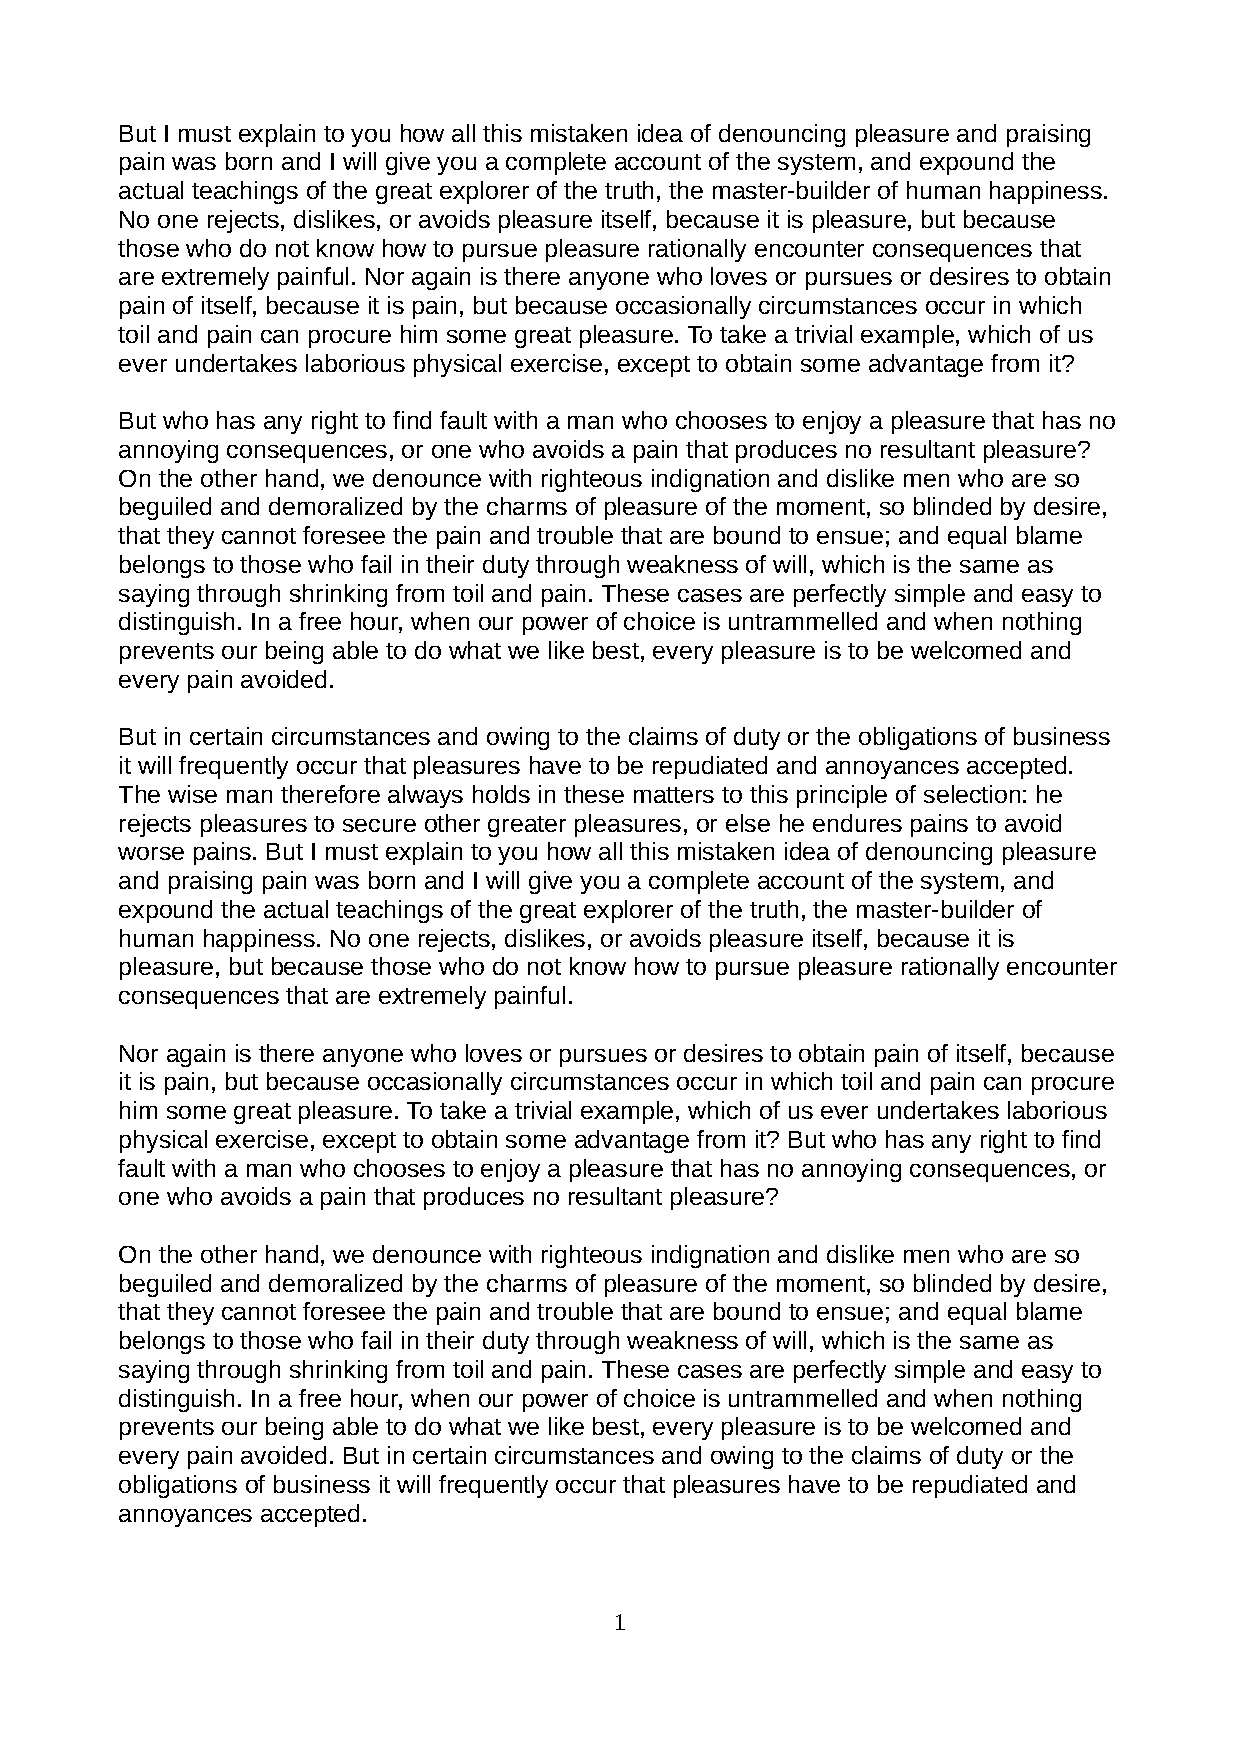
\includegraphics[trim = 0mm 0mm 0mm 0mm,clip, page = 1, width=1\textwidth]{Data/Example_Text.pdf}\\
\end{center}

% all other pages will be included as follows:
\includepdf[pages=2-, pagecommand={}, width=\textwidth]{Data/Example_Text.pdf}
\end{verbatim}

Here, the title page, table of contents, and other documents are included. If they are commented out (\verb|%|), they can be \glqq deleted\grqq{} from the final product.


\paragraph{Directories}

The directories are created once and are to be used repeatedly. Firstly, the sources are included through the \verb|References.bib|, where the citation style (\verb|apacite| for APA-style) is also defined:

\begin{verbatim}
    % References
    \nocite{*}
    \bibliographystyle{apacite}
    \bibliography{References} % bbl, blg files
\end{verbatim}

Afterwards, the list of figures

\begin{verbatim}
    % List of figures
    \listoffigures
    \addcontentsline{toc}{section}{List of Figures}
\end{verbatim}

and the table of tables, where you can also turn on or off a comment.

\begin{verbatim}
    % List of tables
    \listoftables
    \addcontentsline{toc}{section}{List of Tables}
    % Display the comment if needed:
    % \vspace{0.2cm}
    % \noindent
    % ... (see file)
\end{verbatim}

Finally, the code directory:

\begin{verbatim}
    % List of listings
    \lstlistoflistings
    \addcontentsline{toc}{section}{Listings}
\end{verbatim}


\subsubsection{Title Page}

The \verb|titlepage.tex| file is/should be used to design the title page. However, since it mainly contains custom commands as placeholders, there is little need to make changes here. This template can also be used as a template for group assignments. In this case, it can be adapted accordingly (possibly, a separate template for group assignments will also be created).

However, the following commands should be considered for a title page:

\begin{verbatim}
    \begin{titlepage}
        \thispagestyle{empty}
	    \pdfbookmark[1]{Title page}{Title page}
        % ...
    \end{titlepage}
\end{verbatim}

This command defines the title page and removes the header and footer style from this page. In addition, a PDF bookmark can be set for the title page so that the reader can directly click on it later.

\textcolor{red1}{If only the title page is defined, \LaTeX{} creates its own title page!}

\subsubsection{Text}

The text, i.e., the content of the report, is written in the file \verb|text.tex|. How to do this is explained in chapter \ref{sec:examples}. Otherwise, one can also consult the internet. A few small templates can also be found in the additional file \verb|Makros.tex| to ensure consistency. \textcolor{red1}{This file should be replaced by custom commands in the main document to have a consistent environment.}


\subsubsection{References}

The references are saved together in a \verb|References.bib| file. This is a BibTeX file in which one can also write \LaTeX{} code. However, there are a few things to consider.

\begin{verbatim}
    @book{label_bsp_2023,
        author = "Lastname1, Firstname1 AND Lastname2, Firstname2",
        title = {{Example Title}},
        publisher = "Example Publisher",
        year = 2023
    }
\end{verbatim}

This is an example of a book reference. There are also other types of references that have different required and optional attributes.\\

There are also helper programs for this, such as Citavi or \url{https://zbib.org}, but their results must be \textcolor{red1}{\underline{absolutely}} adapted.

How to cite using the packages included and defined here is explained in chapter \ref{sec:citations}.


\subsubsection{Appendix}

The appendix (\verb|appendix.tex|) is used to attach files or materials to the report. For example, assignment descriptions, Python files (and results), as well as other things. One can give each appendix a \verb|\section{}| and also assign a \verb|\label{}| so that one can refer to them in the text. This must start with the following command, after which the appendices can be included:

\begin{verbatim}
    \appendix
    \section{Material} \label{app:material}
\end{verbatim}


\subsection{Software for \LaTeX}

It is recommended to use \href{https://www.overleaf.com/}{www.overleaf.com} or a local program that can compile \LaTeX{} (VSCode, TeXstudio, etc.).

\textcolor{red1}{Please inform yourself how to set it up in each case!}

\pagebreak
\section{Examples} \label{sec:examples}

In this chapter, I would like to discuss the various topics in a scientific paper in the field of \Quotationmarks{Geodesy \& Geoinformatics}:


\subsection{Headings}

Headings are probably the most important means of structuring the content of a paper.

\begin{verbatim}
    \section{Heading}
    \subsection{Subheading}
    \subsubsection{Sub-subheading}
    \paragraph{Paragraph}
\end{verbatim}

For clarity in the document, it is recommended to insert two blank lines before each heading (especially when working with others or sharing your document with others).

In case of overlong headings, the text extends beyond the margin. The following command can help in such cases:

\begin{verbatim}
\section[Heading]{\texorpdfstring{Heading tex}{Heading pdf}}
\end{verbatim}

In this case, the text in the square brackets is responsible for the table of contents, while the other strings control the formatting and display in the PDF.


\subsection{Text-formatting}

Text can also be formatted as \textit{italic}, \textbf{bold}, \textbf{\textit{bold \& italic}}, and \underline{underlined}.

\begin{verbatim}
    \textit{italic}
    \textbf{bold}
    \textbf{\textit{bold & italic}}
    \underline{underlined}
\end{verbatim}

But text can also be changed in size:\\

\verb|\Huge| \hfill {\Huge Huge}

\verb|\huge| \hfill {\huge huge}

\verb|\LARGE| \hfill {\LARGE LARGE}

\verb|\Large| \hfill {\Large Large}

\verb|\large| \hfill {\large large}

\verb|\small| \hfill {\small small}

\verb|\footnotesize| \hfill {\footnotesize footnotesize}

\verb|\scriptsize| \hfill {\scriptsize scriptsize}

\verb|\tiny| \hfill {\tiny tiny}\\

The command can be enclosed either in curly brackets \verb|{\LARGE Text}| or in a command:

\begin{center}
    \begin{LARGE}
        LARGE
    \end{LARGE}
\end{center}

\begin{verbatim}
    \begin{center}
        \begin{LARGE}
            LARGE
        \end{LARGE}
    \end{center}
\end{verbatim}


\subsubsection{Text Color}

To display text in a different color, the command \verb|\textcolor{color}{text}| is used. The color is defined in the main document.

\textcolor{HCU}{I am in HCU blue.}\\
\textcolor{red1}{I am in red.}\\
\textcolor{mygray}{I am gray.}

\begin{verbatim}
    \textcolor{HCU}{I am in HCU blue.}\\
    \textcolor{red1}{I am in red.}\\
    \textcolor{mygray}{I am gray.}
\end{verbatim}

Alternatively, the new command \verb|\HCUcolor{}| can be used:

\HCUcolor{I am in HCU blue.}


\subsubsection{Quotation Marks}

"This is in normal quotation marks." And here is normal text.

\glqq This is in correct quotation marks.\grqq{} And here is normal text.

\begin{verbatim}
"This is in normal quotation marks." And here is normal text.

\glqq This is in correct quotation marks.\grqq{} And here is normal text.
\end{verbatim}

Thus, one can use \verb|\glqq| for opening and \verb|\grqq{}| (brackets important for spacing) for closing quotation marks.\\

Or one can use the new command \verb|\Quotationmarks{}|:

\Quotationmarks{I am in quotation marks.}


\subsection{Paragraphs}

Option 1 as shown in section \ref{sec:simple-paragraph}:

\begin{verbatim}
    Here is paragraph 1.
    % There is an empty line in between (this is just a comment)
    Here is paragraph 2.
\end{verbatim}

Option 2 as shown in section \ref{sec:clear-paragraph}:

\begin{verbatim}
    Here is paragraph 1.\\
    % There is an empty line in between (this is just a comment)
    Here is paragraph 2.
\end{verbatim}

Option 2 looks better.


\subsubsection{Simple paragraph formation} \label{sec:simple-paragraph}

Pain is a complex and subjective experience that is difficult to define. While it is generally seen as an unpleasant sensation, it can also have positive associations, such as signaling healing or growth. However, most people try to avoid pain whenever possible, and it is often associated with negative emotions like fear, anxiety, and sadness. % Paragraphs can be formed by a blank line or ...

Despite its negative associations, pain serves an important function in alerting us to potential danger or harm. It can also motivate us to take action to alleviate the pain and prevent further injury. Overall, while pain is not something we seek out, it is an integral part of the human experience.

\subsubsection{Clearer paragraph formation} \label{sec:clear-paragraph}

Pain is a complex and subjective experience that is difficult to define. While it is generally seen as an unpleasant sensation, it can also have positive associations, such as signaling healing or growth. However, most people try to avoid pain whenever possible, and it is often associated with negative emotions like fear, anxiety, and sadness.\\ % ... two paragraphs can also be visually separated more from each other

Despite its negative associations, pain serves an important function in alerting us to potential danger or harm. It can also motivate us to take action to alleviate the pain and prevent further injury. Overall, while pain is not something we seek out, it is an integral part of the human experience.


\subsection{Referencing}

As shown in Chapter \ref{sec:firstSec}, it is possible to set different headings and write the text. Now you already have a label and a reference set. Here are a few examples of labels:

\begin{verbatim}
    \label{sec:heading}
    \label{fig:figure}
    \label{tab:table}
    \label{eq:formula}
    \label{lst:listing}
    \label{app:appendix}
\end{verbatim}

The abbreviations at the beginning provide a clearer assignment, but they are not mandatory. These can be referenced with \verb|\ref{label}|, but \verb|\autoref{label}| is also possible, although the latter does not always provide the desired output. For example, \verb|\autoref{}| is helpful when referring to figures or tables in the text, as it also adds the type of object. However, headings are not prefixed with a correct object type:

\autoref{fig:HCU-logo}, \autoref{tab:Test}, \autoref{sec:examples} or chapter \ref{sec:examples}\\

If you want to refer to them in brackets, you can use \verb|\ref{}| again:

(Fig. \ref{fig:HCU-logo}, Tab. \ref{tab:Test}, Chap. \ref{sec:examples})


\subsection{Citations} \label{sec:Citations}

I like to quote from a specialized book \cite[p. xx ff.]{9783879076581}. Or directly \citeA[p. xx ff.]{9783879076581}.

\begin{verbatim}
    \cite[p. xx ff.]{example_label_2023} % indirect
    \citeA[p. xx ff.]{example_label_2023} % direct
\end{verbatim}

But if you have two sources, you can also combine the individual attributes:

\begin{verbatim}
    (\citeauthor{9783879076581}, \citeyearNP{9783879076581}, p. xx; ...)
\end{verbatim}

(\citeauthor{9783879076581}, \citeyearNP{9783879076581}, p. xx; ...)


\subsection{Figures}

Figures can be implemented as follows:

\begin{figure}[H]
    \centering
    
\includegraphics[width=0.75\textwidth]{Data/hcu_logo.pdf}
    \caption{HCU logo}
    \caption*{Source: } % a source can be specified using \citeA[p. ]{}
    \label{fig:HCU-logo}
\end{figure}

It is recommended to leave a blank line between paragraphs and figures.

\begin{verbatim}
    \begin{figure}[H]
        \centering
        \includegraphics[width=0.75\textwidth]{Data/File}
        \caption{Caption}
        \caption*{Source: \citeA[p. xx]{}}
        \label{fig:my_label}
    \end{figure}
\end{verbatim}

The \verb|[H]| needs to be set to ensure that the figure is inserted exactly there. Additional options can be specified in the square brackets of the\linebreak \verb|\includegraphics[options]{path/filename}| command.\\

With a short command (see \textit{README.md} or \textit{main document}) you can insert the above image as follows:

\begin{verbatim}
    \figureWithSource{hcu_logo.pdf}{HCU-Logo}{Source}{HCU-logo}
\end{verbatim}


\subsubsection{Two Figures}

Sometimes it is desirable to display two figures side-by-side. This can be achieved using subfigures:

\begin{verbatim}
    \begin{figure}[H]
        \begin{subfigure}[c]{0.48\textwidth}
            \includegraphics[width=\textwidth]{Data/}
            \subcaption{}
            \label{fig:}
        \end{subfigure}
        \hfill
        \begin{subfigure}[c]{0.48\textwidth}
            \includegraphics[width=\textwidth]{Data/}
            \subcaption{}
            \label{fig:}
        \end{subfigure}
        \caption{}
        \caption*{Source: \citeA[]{}}
        \label{fig:}
    \end{figure}
\end{verbatim}


\subsection{Tables}

Tables cannot be created as easily in \LaTeX{} as in Word or Excel. The easiest way is to create an Excel file with all the calculations and then paste it into \href{https://www.tablesgenerator.com/latex_tables}{TableGenerator} using File ... Paste table data ..., then adjust as needed. Afterwards, the code for \LaTeX{} can be generated and inserted. Additional options for headers, labels, and layout can also be defined.

\begin{table}[H]
    \centering
    \begin{tabular}{|c|c|c|}
        \hline
        This    & is        & just  \\ \hline
        a       & little    & test  \\ \hline
        for     & \LaTeX{}  & !!!   \\ \hline
    \end{tabular}
    \caption{Test Table} \label{tab:Test}
    \caption*{source can also be added here}
\end{table}

Das \verb|[H]| muss noch gesetzt werden, damit die Tabelle genau dort eingefügt wird und das Layout besser aussieht. Die \autoref{tab:Test} sieht als Code wie folgt aus:

\begin{verbatim}
    \begin{table}[H]
        \centering
        \begin{tabular}{|c|c|c|}
            \hline
            This    & is        & just  \\ \hline
            a       & little    & test  \\ \hline
            for     & \LaTeX{}  & !!!   \\ \hline
        \end{tabular}
        \caption{Test Table} \label{tab:Test}
        \caption*{source can also be added here}
    \end{table}
\end{verbatim}


\subsection{Formulas}

There are several options here. In the text:\\
The Pythagorean theorem is: $c^2 = a^2 + b^2$. \\
Just like that, which is not recommended: \\
\[\label{eq:GaussianErrorIntegral}
\int_{-\infty}^{+\infty} e^{-x^2} dx = \sqrt{\pi} \cdot \frac{1}{2}
\]

Or like this, which is highly recommended:

\begin{equation}
	\numberwithin{equation}{section}
	c^2 = a^2 + b^2 \label{eq:Pythagoras} \\
\end{equation}

\begin{verbatim}
    \begin{equation}
        \numberwithin{equation}{section}
        Formel \label{eq:formula} \\
    \end{equation}
\end{verbatim}

It is also helpful to use a \href{https://www.codecogs.com/latex/eqneditor.php}{formula editor}.\\

When working with matrices (or vectors) or words within formulas, it is recommended to use \verb|\mathbf{}| for matrices (or vectors) and \verb|\text{}| or \verb|\textbf{}| for words. For example:

\begin{equation}
	\numberwithin{equation}{section}
	\mathbf{\hat{x}} = \mathbf{\left(A^T A\right)}^{-1} \mathbf{A^T \ell} \label{eq:adjustment} \\
\end{equation}

\begin{equation}
	\numberwithin{equation}{section}
	M = \frac{\text{map distance}}{\text{distance in nature}} = \frac{s_K}{s_N} = \frac{1}{m} \label{eq:scale} \\
\end{equation}


\subsection{Listings (Python Code)}

Python code can be included in \LaTeX{} documents in two different ways. The first option is to directly include the code in the document as shown below:

\begin{lstlisting}[language=Python, style=Python, caption=Basemap-Anwendung, label={lst:basemap}]
	# Libraries
	from mpl_toolkits.basemap import Basemap
	import matplotlib.pyplot as plt
	# Initialize the map
	map = Basemap(llcrnrlon=-160, llcrnrlat=-60, urcrnrlon=160, urcrnrlat=70)
	# Continent and countries!
	map.drawmapboundary(fill_color="#A6CAE0")
	map.fillcontinents(color="#e6b800", lake_color="#e6b800")
	map.drawcountries(color="white")
	plt.show()
\end{lstlisting} 

or else from an existing file

\lstinputlisting[language=Python, style=Python, firstline=17, lastline=26, caption=TCP-Server, label={lst:tcpserver}]{Data/03_tcp_server.py}


\subsection{Bullet Lists}

Bullet lists can be used for the inventory:

\begin{itemize}	
	\setlength{\itemsep}{-2pt} % here the distance can be chosen
	\item Trimble S7 (serial number: VE72)
	\item 2 reflectors with tripod and optical plumb
	\item 3 tripods
\end{itemize}

\begin{verbatim}
    \begin{itemize}	
    	\setlength{\itemsep}{-2pt} % here the distance can be chosen
    	\item Trimble S7 (serial number: VE72)
    	\item 2 reflectors with tripod and optical plumb
    	\item 3 tripods
    \end{itemize}
\end{verbatim}

However, if no distance is specified, it looks like this:

\begin{itemize}	
	\item Trimble S7 (serial number: VE72)
	\item 2 reflectors with tripod and optical plumb
	\item 3 tripods
\end{itemize}

Therefore, it is advisable to reduce this distance. Additional text can also be inserted under each point as if one were creating a paragraph (\verb|\\|):

\begin{itemize}	
	\setlength{\itemsep}{-2pt} % here the distance can be chosen
	\item Trimble S7 (serial number: VE72)\\
	Here is some additional text.
	\item 2 reflectors with tripod and optical plumb
	\item 3 tripods
\end{itemize}

This can also be formulated as follows with a standardized command:

\begin{verbatim}
    \ownItems{
        \item Trimble S7 (serial number: VE72)\\
        Here is some additional text.
        \item 2 reflectors with tripod and optical plumb
        \item 3 tripods
    }
\end{verbatim}


\subsection{Spacing}

Spacing can be adjusted both horizontally and vertically, and can also be filled. Sometimes it is necessary to adjust spacing for better layout:

Text on the left \hfill but also on the right.

\vspace{10mm}
{\hfill One centimeter below on the right side.}

\begin{verbatim}
    Text on the left \hfill but also on the right.

    \vspace{10mm}
    {\hfill One centimeter below on the right side.}
\end{verbatim}

The commands are \verb|\hfill|, \verb|\vfill|, \verb|\hspace{}| and \verb|\vspace{}|, whereby the latter two can also be written with an asterisk (\verb|*|) between the command and the brackets if you want to force the spacing.

\pagebreak
\subsection{Minipages}

Sometimes it's better to place text and images side by side. Here, two \verb|minipage| are useful:\\

\begin{minipage}[H]{0.48\textwidth}
	There is no one who loves pain itself, who seeks after it and wants to have it, simply because it is pain, unless it is to occur in some circumstances in which toil and pain can procure him some great pleasure. To take a trivial example, which of us ever undertakes laborious physical exercise, except to obtain some advantage from it?
\end{minipage}
\hfill
\begin{minipage}[H]{0.48\textwidth}
	There is no one who loves pain itself, who seeks after it and wants to have it, simply because it is pain, unless it is to occur in some circumstances in which toil and pain can procure him some great pleasure. To take a trivial example, which of us ever undertakes laborious physical exercise, except to obtain some advantage from it?
\end{minipage}\\

\begin{verbatim}
    \begin{minipage}[H]{0.48\textwidth}
    	
    \end{minipage}
    \hfill
    \begin{minipage}[H]{0.48\textwidth}
    	
    \end{minipage}\\
\end{verbatim}

More than two minipages can also be placed side by side. The column width should never add up to 1, and a horizontal distance is also useful for a beautiful layout. Almost everything can be used or designed in minipages as usual. It is recommended to make a paragraph (\verb|\\|) before and after.


\subsection{Columns}

Columns are rather not that useful, unless you don't want to use a minipage, because here the content is divided evenly:

\begin{multicols}{2}
	There is no one who loves pain itself, who seeks after it and wants to have it, simply because it is pain, unless it is to occur in some circumstances in which toil and pain can procure him some great pleasure. To take a trivial example, which of us ever undertakes laborious physical exercise, except to obtain some advantage from it? There is no one who loves pain itself, who seeks after it and wants to have it, simply because it is pain, unless it is to occur in some circumstances in which toil and pain can procure him some great pleasure. To take a trivial example, which of us ever undertakes laborious physical exercise, except to obtain some advantage from it?
\end{multicols}

\begin{verbatim}
    \begin{multicols}{2}
    	
    \end{multicols}
\end{verbatim}

Here, too, the number of columns can be increased:

\begin{multicols}{3}
	There is no one who loves pain itself, who seeks after it and wants to have it, simply because it is pain, unless it is to occur in some circumstances in which toil and pain can procure him some great pleasure. To take a trivial example, which of us ever undertakes laborious physical exercise, except to obtain some advantage from it? There is no one who loves pain itself, who seeks after it and wants to have it, simply because it is pain, unless it is to occur in some circumstances in which toil and pain can procure him some great pleasure. To take a trivial example, which of us ever undertakes laborious physical exercise, except to obtain some advantage from it?
\end{multicols}


\subsection{Embed PDF pages}

If you want to add a PDF page, as for the attachment, so that there is no blank page, use the command included in \verb|Makros.tex|.\\

If you want to insert a PDF as a raster, for example presentation slides, the command \verb|\includepdf[options]{filepath}| is recommended (see \verb|Makros.tex|). There you can define the PDF pages and the raster (\verb|nup=<columns>x<rows>|). The command \verb|pagecommand={}| preserves the header and footer.


\subsection{Different breaks}

If a page is well-formatted and a page break should occur, one of the following commands can be used:

\begin{verbatim}
    \pagebreak
    \newpage
\end{verbatim}

If a line break is desired instead, the following command is recommended:

\begin{verbatim}
    \linebreak
\end{verbatim}


\subsection{Comment}

To leave comments to yourself or your co-authors while writing, you can use the following command:

\begin{verbatim}
    \ownComment{Here is a comment.}
\end{verbatim}

This command is then displayed as follows and must be commented out or deleted \textbf{\underline{before submission}}:

\ownComment{Here is a comment.}


\vfill
\section{Closing Words}

These were a lot of impressions in \LaTeX{} and I hope this template will help you.\\

If you have any questions, feel free to write to me or create an issue on GitHub. Thank you very much!

Also, make sure to check GitHub regularly!\\

Have fun writing and good luck with your studies.

Fabian Bloch

\vspace{7mm}
\textcolor{HCU}{P.S.: You can also upload a ZIP file to Overleaf via \glqq New Project... Upload Project\grqq{}.}